\documentclass[11pt]{book}              % Book class in 11 points

%\parindent0pt  \parskip10pt             % make block paragraphs
%\raggedright                            % do not right justify

\usepackage[margin=1in]{geometry}



\usepackage{amssymb,amsmath,bm}
\usepackage{graphicx,subfigure,epsfig,color}
\usepackage{url,hyperref}
\usepackage{algpseudocode,algorithm}
\usepackage{array,multirow}
\usepackage[noadjust]{cite}
\usepackage[normalem]{ulem}

\newtheorem{assumption}{Assumption}
\newtheorem{theorem}{Theorem}
\newtheorem{corollary}{Corollary}
\newtheorem{definition}{Definition}
\newtheorem{lemma}{Lemma}
\newtheorem{proposition}{Proposition}
\newtheorem{remark}{Remark}
\newtheorem{example}{Example}	
\newenvironment{scase}[1][Special Case]{\begin{trivlist}
\item[\hskip \labelsep {\bfseries #1}]}{\end{trivlist}}


%My Macros
\newcommand{\algorithmicbreak}{\textbf{break}}
\newcommand{\Break}{\State \algorithmicbreak}
\newcommand{\algorithmiccontinue}{\textbf{continue}}
\newcommand{\Continue}{\State \algorithmiccontinue}
\newcommand{\algorithmicand}{\textbf{and }}
\renewcommand{\And}{\algorithmicand}
\newcommand{\Real}{\mathbb R}
\newcommand{\Borel}{\mathcal B}
\newcommand{\Natural}{\mathbb N}
\newcommand{\Prob}{\mathbb P}
\newcommand{\Normal}{\mathcal N}
\newcommand{\Identity}{\mathbb I}
\newcommand{\Expected}[1]{\mathbb{E}\left[#1\right]}
\newcommand{\imag}{\text{i }}
\newcommand{\Trace}{\mathbf{Tr}}
\newcommand{\etal}{\textit{et al. }}
\newcommand{\eqnref}[1]{(\ref{#1})}
\newcommand{\Eqnref}[1]{Eqn.\ (\ref{#1})}
\newcommand{\Fig}[1]{Figure \ref{#1}}
\newcommand{\fig}[1]{Fig. \ref{#1}}

\renewcommand{\v}[1]{\ensuremath{\mathbf{#1}}}
\newcommand{\vo}[1]{\ensuremath{\boldsymbol{#1}}}
\newcommand{\pderiv}[2]{\frac{\partial #1}{\partial #2}}
\newcommand{\half}{\frac{1}{2}}
\newcommand{\prob}[1]{\mathbf{P}\left(#1\right)}

\renewcommand{\v}[1]{\ensuremath{\mathbf{#1}}}
\renewcommand{\citepunct}{, } % Was {], [}
\renewcommand{\citedash}{--}  % Was {]--[}
\newcommand{\M}[2]{M^{#1-}_{#2}}
\newcommand{\tabref}[1]{ Table \ref{#1}}
\newcommand{\y}{\tilde{y}}

\newcommand{\vv}[2]{\left( \begin{array}{c} #1\\#2\end{array}\right)}
\newcommand{\Mat}[4]{\left( \begin{array}{cc} #1 & #2 \\#3 & #4 \end{array}\right)}


% Note that book class by default is formatted to be printed back-to-back.
\begin{document}                        % End of preamble, start of text.
\frontmatter                            % only in book class (roman page #s)
\begin{titlepage} 
	\centering
	{\huge\bfseries The National Airspace Trajectory-Prediction System\par}
	\vspace{1cm}
	{\huge\bfseries Algorithm Glossary\par}	
	\vspace{3.5cm}
	{Report prepared under NASA University Leadership Initiative Project\par}
	\vfill
	Dr. P.K.Menon, Dr. Parikshit Dutta, Oliver Chen, Hari Iyer and Dr. Bong-Jun Yang\par
	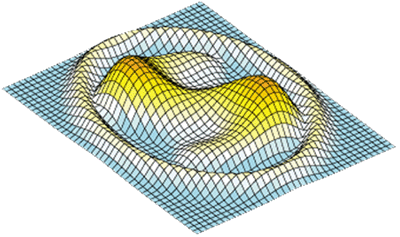
\includegraphics[width=0.4\textwidth]{Pictures/companylogo.png}\par
%	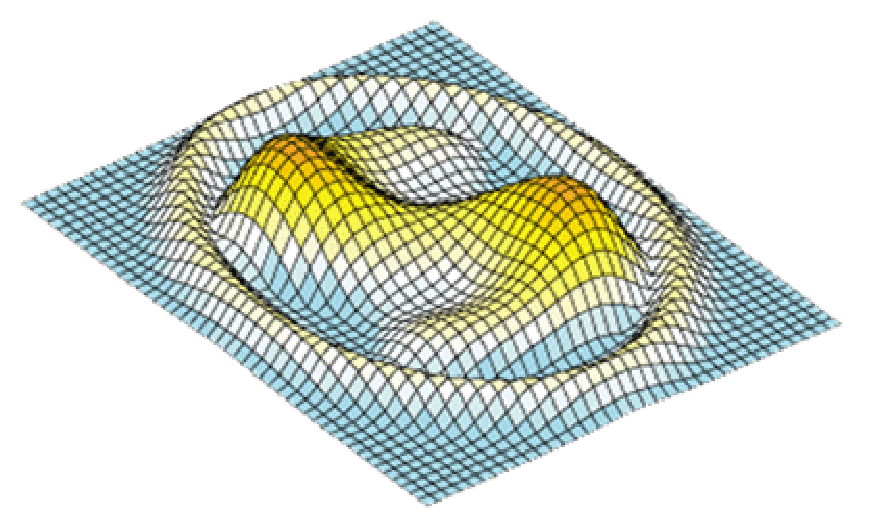
\includegraphics[width=0.4\textwidth]{Pictures/companylogo.eps}\par
	{\itshape Optimal Synthesis Inc., Suite 240,\par Los Altos, CA, 94022.\par}
	\vfill
% Bottom of the page
	{\large \today\par}
\end{titlepage}
\tableofcontents                        % Print table of contents
\mainmatter                             % only in book class (arabic page #s)
\chapter{Introduction}                % Print a "chapter" heading
Overview of NATS and the interfaces and what will the book contain. 
%%%%%%%%%%%%%%%%%%%%%%%%%%%%%%%%%%%%%%%%%%%%%%%%%%%%%%%%%%%%%%%%%%%%%%%
\chapter{Overall Architecture}
The NATS software is designed to simulate ensemble of aircraft trajectories starting from the departure gate to the arrival gate. It is designed on a server-client framework. The server hosts all the databases, models and algorithms. The client connect with the server and invokes the simulation. Once the simulation is over, the client can access simulation outputs for post processing. \par
%%%%
At its core, the NATS consists of three interfaces: equipment interface, environment interface and entity interface. Each interface interacts with other to create the gate-to-gate air traffic simulation. Further, at any given time the overall system-wide safety of the National Airspace System (NAS) can be investigated via a safety metric interface. \par
%%
This Chapter describes the overall NATS architecture and its critical components. 
\section{The Server-Client Model}
The NATS trajectory propagation engine is based on a Server-Client model. The server contains the aircraft performance models, the airspace procedures, terrain, wind and weather data as well as the algorithms for propagation. The client creates flight plans for aircraft to be simulated and invokes the simulation by sending the flight plan data to the server.
The client is available to users and can be used on multiple platforms such as Python, Java\texttrademark and Matlab\textregistered.\par
%%%%%%%%%%%%%%%%%%
The basic structure of NATS is shown in \Fig{fig:NATSbasic}. A remote server, which hosts NATS models and databases, can be accessed by users through NATS client. The client inputs flight plans and initial states of the flights to be simulated. It is sent to the remote server where the NATS simulation is run. The trajectory outputs can be then visualized in the client side using interface of the user's choice.
\begin{figure}[H]
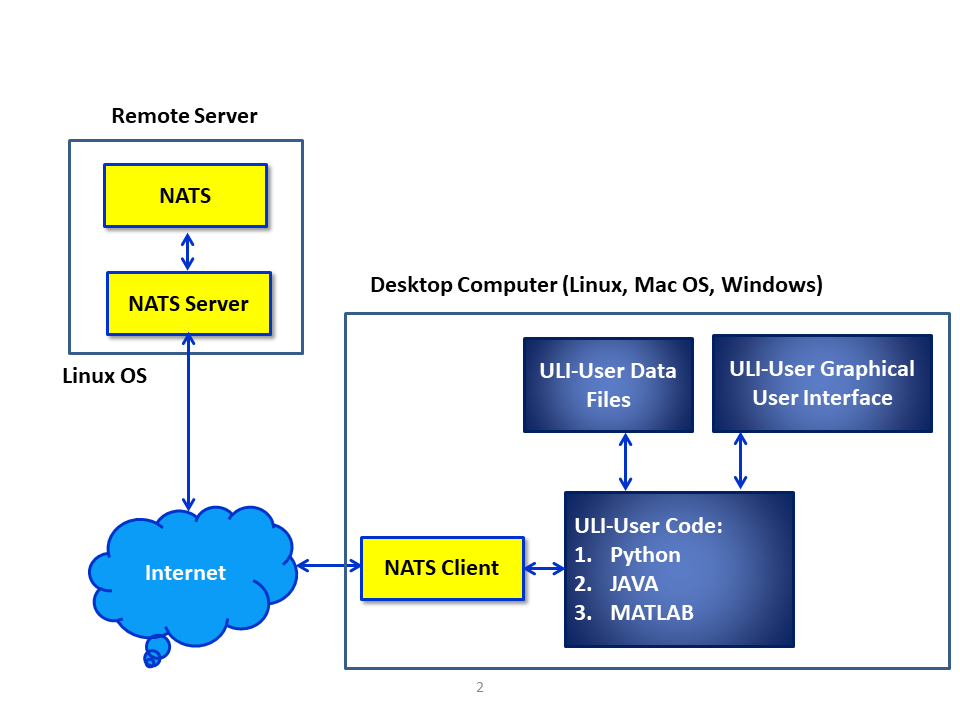
\includegraphics[width=0.9\textwidth]{Pictures/Slide2.PNG}
%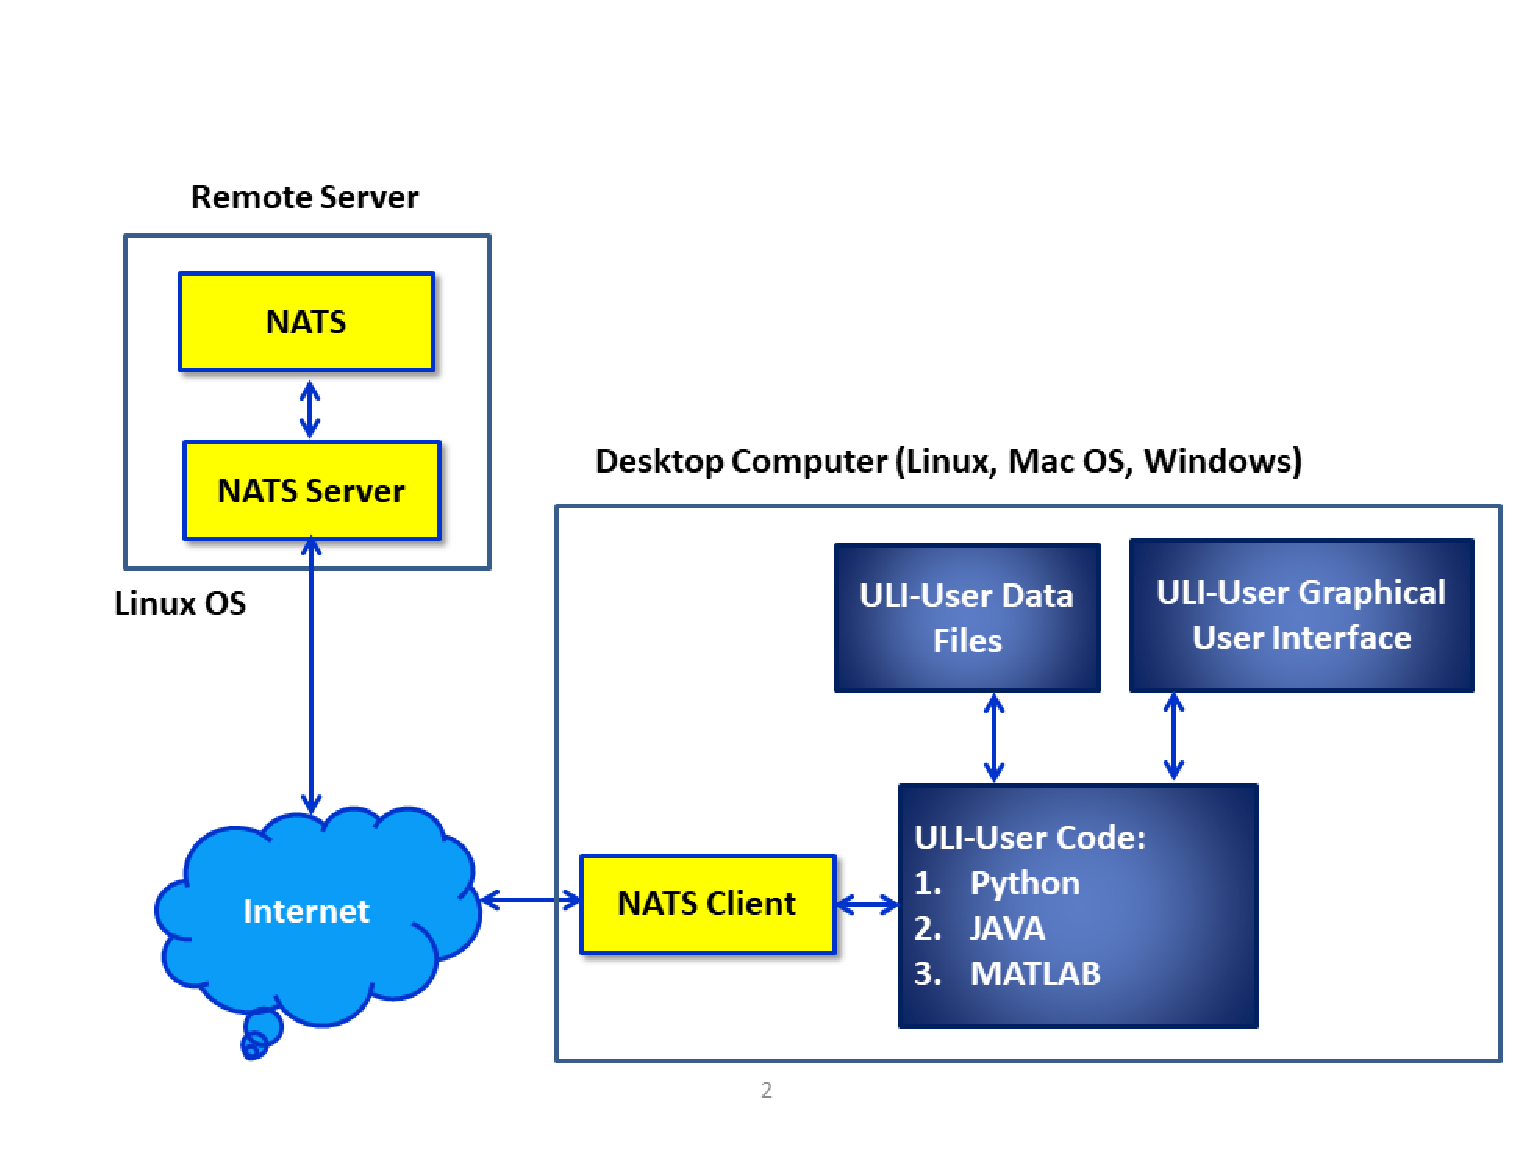
\includegraphics[width=0.9\textwidth]{Pictures/Slide2.eps}
\caption{The Basic Structure of NATS. \label{fig:NATSbasic}}
\end{figure}
The projected final structure of NATS is shown in \Fig{fig:NATSfinal}. Multiple users will be able to connect with NATS from different places at the same time. Further, real-time simulations with feedback from ADS-B can be inputted to NATS. Moreover, users will be able to  connect virtual aircraft simulators such as x-planes to NATS. The server then would take all the user inputted aircraft and simulate them as an ensemble.
\begin{figure}[H]
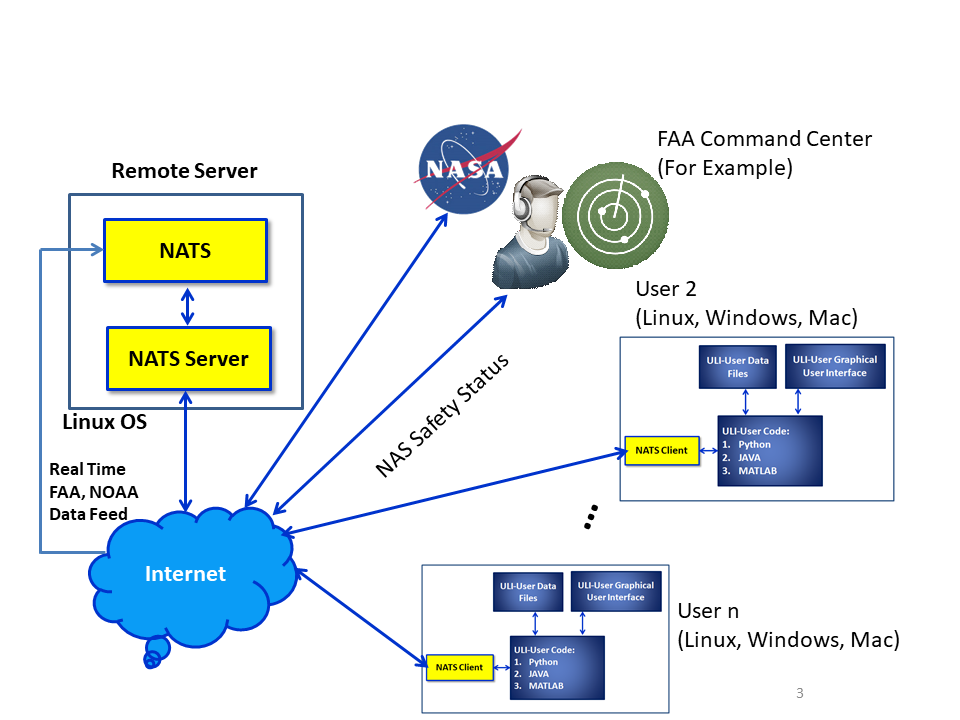
\includegraphics[width=0.9\textwidth]{Pictures/Slide3.PNG}
%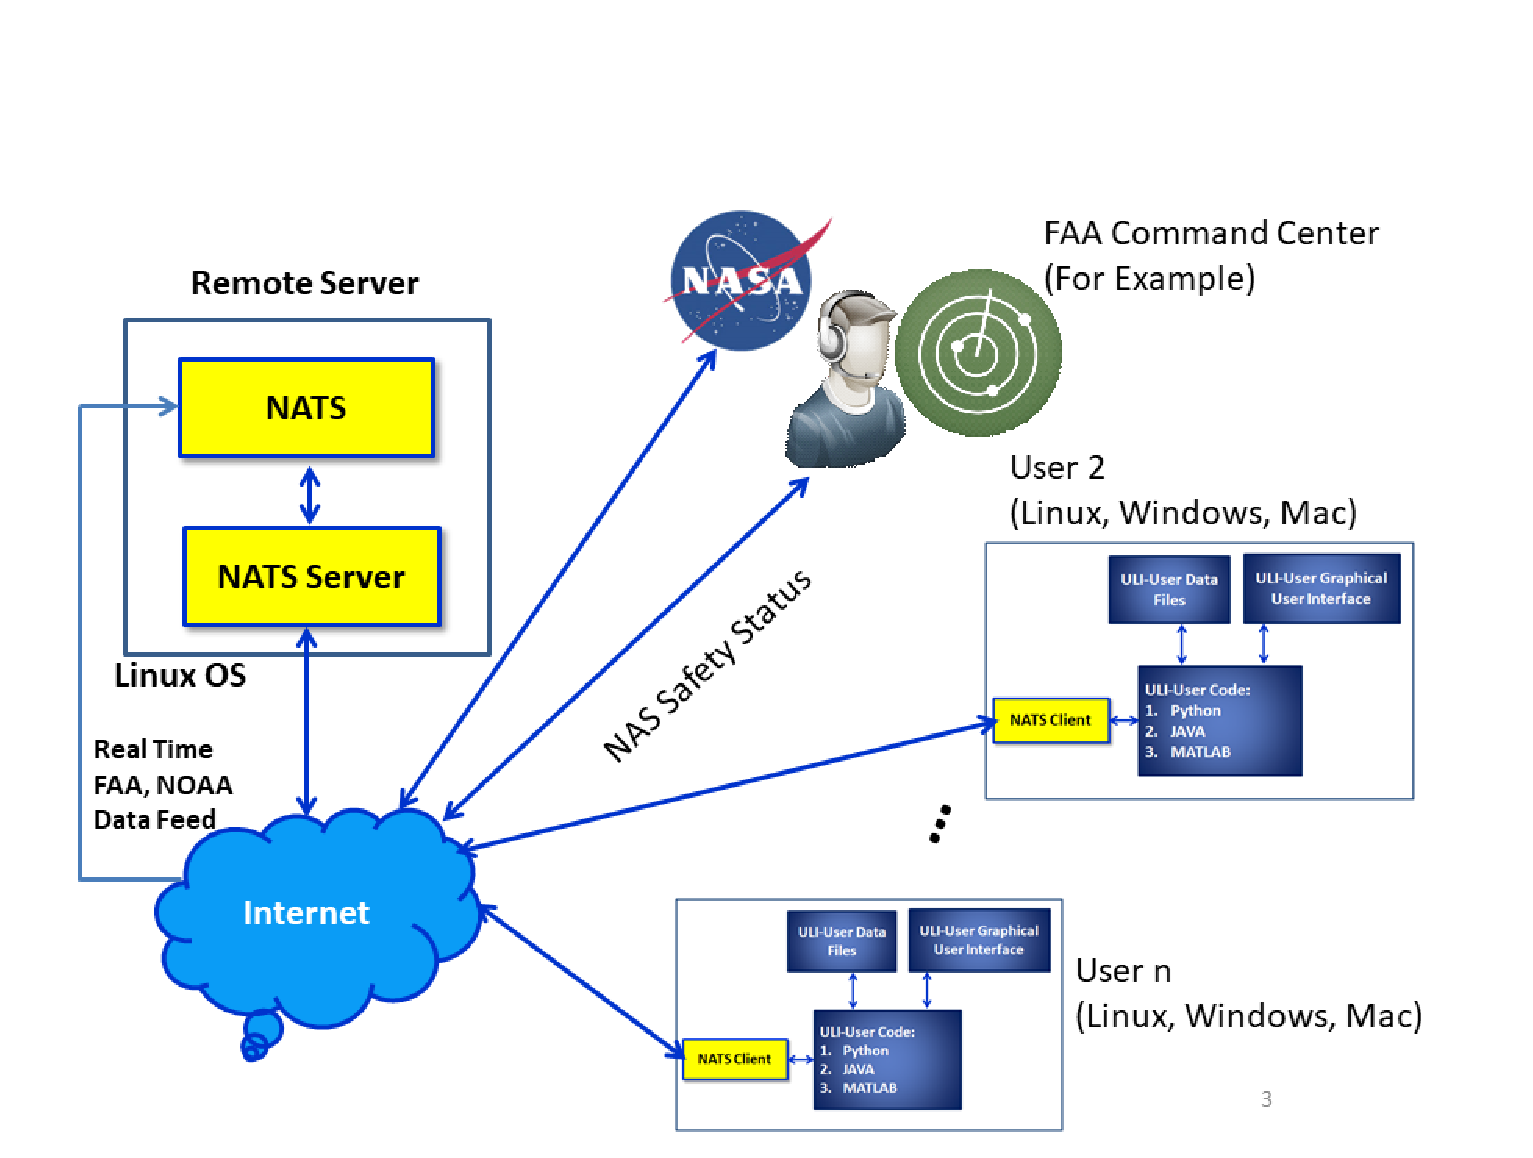
\includegraphics[width=0.9\textwidth]{Pictures/Slide3.eps}
\caption{The Projected Capabilities of NATS. \label{fig:NATSfinal}}
\end{figure}

\section{NATS Interfaces}
NATS software module is consists of three interfaces which interact with each other: 
\begin{itemize}
\item \textbf{Equipment Interface}: Consists of the aircraft itself, communication and navigation systems, ground vehicles, flight deck systems etc.
\item \textbf{Environment Interface}: Consists of the airports, terrain, surface winds, weather and the operating procedures laid out by FAA. 
\item \textbf{Entity Interface}: Consists of the pilots, controllers and the ground oeprating staff.
\end{itemize}
The entire system has been described in \Fig{fig:natsinterfaces}.The NATS sofware framework is designed such that these contributing modules interact with each other to create a gate-to-gate air traffic simulation software. 
\begin{figure}[H]
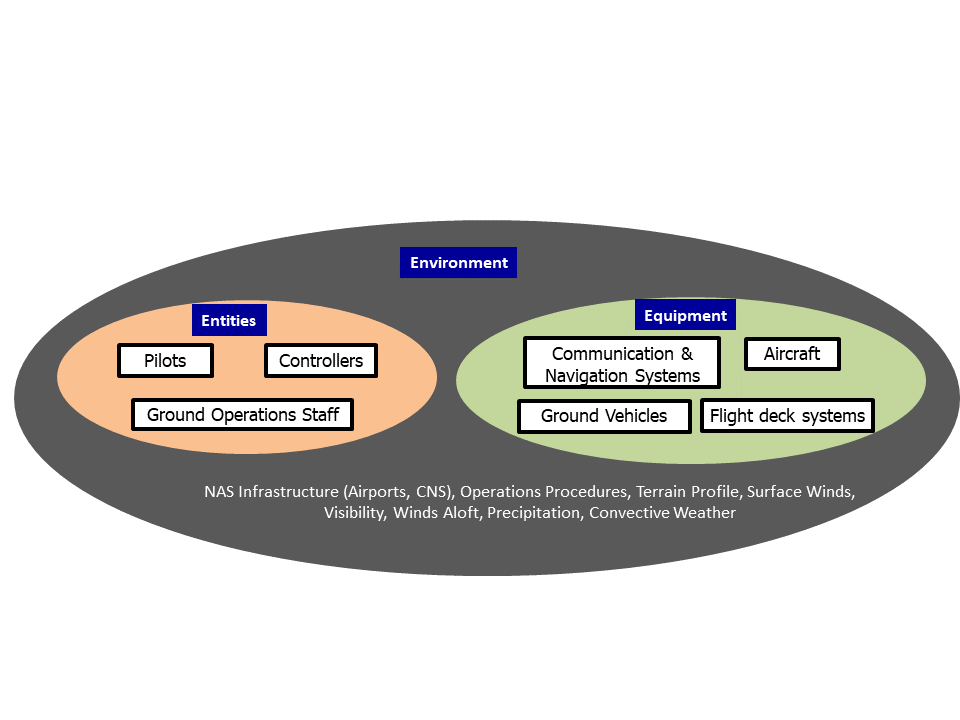
\includegraphics[width=0.9\textwidth]{Pictures/Slide1.PNG}
%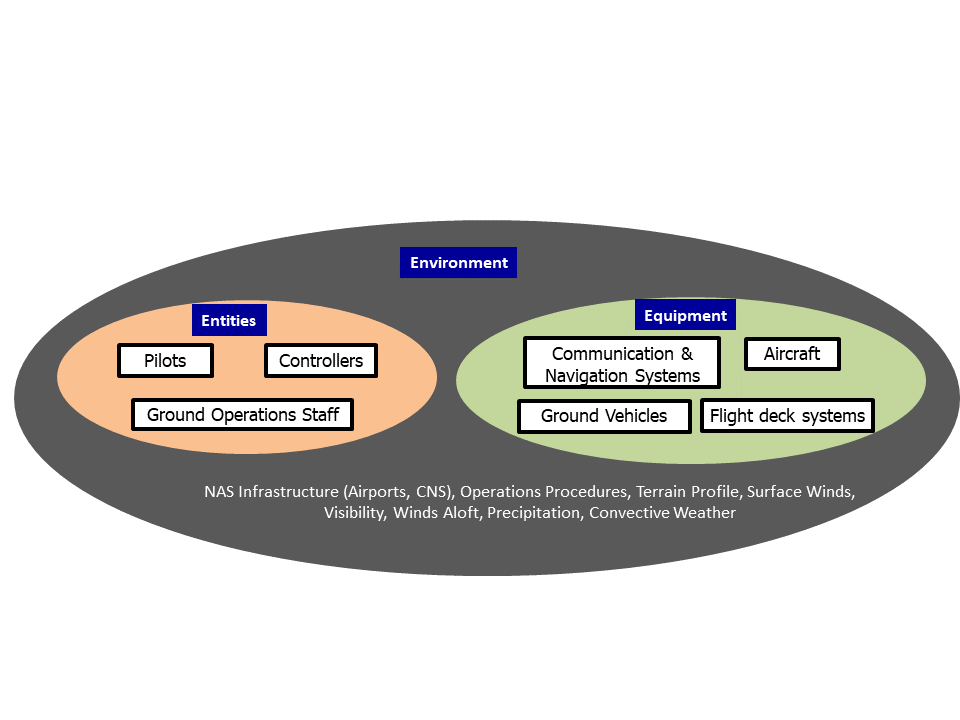
\includegraphics[width=0.9\textwidth]{Pictures/Slide1.eps}
\caption{Different Components of the NATS Software.\label{fig:natsinterfaces}}
\end{figure}
The NATS software allows the user to access individual members of each interface and modify their properties before and during simulation.
\subsection{Equipment Interface}
As indicated in the Introduction section, the main equipments employed in the NAS are aircraft together with flight-deck automation system, ground service vehicles, communication systems, and surveillance systems. Although it may be desirable to incorporate high-fidelity models
describing their nominal and off-nominal behaviors, this may not be feasible due to large number of subsystems that needs to be included, leading to unmanageable computational effort. Consequently, simpler models capturing the essential features of their operation are included. The following subsections provide additional details.
\subsubsection{Aircraft and Ground Vehicle Models}
High-fidelity aircraft models are generally described a set of 12 first-order nonlinear differential equations. However, six of these are not relevant to the system safety analysis,
because they deal with the attitude motions of the aircraft in flight. Eliminating these equations from the aircraft dynamics is equivalent to assuming that the aircraft are always in “moment equilibrium”. Under this assumption the aircraft dynamics can be described by six first-order nonlinear ordinary differential equations, commonly termed as the point-mass model. These equations generally require detailed knowledge about the aircraft engines, aerodynamics
and mass.
Since it is nearly impossible to get accurate data for every
aircraft that are operating in the NAS, a further
simplification is made in the analysis. The simplification
consists of employing the three differential equations
describing the position kinematics of aircraft, together with
rate of climb, rate of descent, and airspeed or Mach number
bounds from well-known databases such as BADA \cite{BADA}. This database was assembled by
Eurocontrol using actually observed trajectories in the
European airspace.\par
With these simplifications, the equations of motion for an
aircraft are given by:
\begin{eqnarray}
\dot{h} &=&f(h,A)\\
\dot{\lambda}&=& \frac{1}{R_e+h}\left( V\cos\gamma\cos\chi+W_N \right)\\
\dot{\tau} &=& \frac{1}{(R_e+h)\cos\lambda}\left( V\cos\gamma\sin\chi+W_E \right)
\end{eqnarray}
where, $h$ is the altitude of the aircraft, $\lambda$ is the latitude and $\tau$ is the longitude. Further, the instantaneous flight path angle can be found from $\gamma = \sin^{-1}(\dot{h}/V)$, where $V_{\min}\leq V(h,A)\leq V_{\max}$.\par

The control variables in this model are the airspeed $V$, flight path angle $\gamma$ or the altitude rate $f(h,A)$, and the course angle $\chi$. Note that the limits on the climb and descent rates and the airspeed are specified in BADA for over 400 Aircraft types. In the present NATS framework, these variables are chosen by the human pilot and/or flight deck
automation to follow flight plans approved by the controller.The North component of the wind $W_N$ and the East component of the wind $W_E$ are obtained from the NOAA weather data.\par

In order to enable the investigation of potential accidents and incidents that can occur in each flight phase, the aircraft operations in the NAS have been separated into 11 major
flight regimes. These are: stationary at the gate, pushback, taxi to runway, takeoff, climbout, climb-to-cruise, cruise, initial descent, approach, landing, taxi to gate. The software is designed such that the salient motion characteristics of aircraft in historic accidents and incidents in each of these flight regimes and their impact on NAS operations can be formulated and analyzed.\par 

The motion of the aircraft on the ground and the motion of ground vehicles can be simulated by eliminating the altitude dynamics, and assuming that the flight path angle $\gamma$ is zero. Moreover, the wind has negligible effect on aircraft motion when it is on the ground. With these simplifications, the equations of motion for the aircraft moving on the ground, and the equations of motion for the ground vehicle, are:
\begin{eqnarray}
\dot{\lambda}&=& \frac{V\cos\chi}{R_e+h}\\
\dot{\tau} &=& \frac{V\sin\chi}{(R_e+h)\cos\lambda}
\end{eqnarray}
The control variables employed by the pilot or the ground vehicle are the speed V and the course angle $\chi$ used to move along the ramp, taxiways, and up to the runway. The aircraft and ground vehicle dynamic equations are integrated using the first-order Euler integration method.
\subsubsection{Navigation and Flight-Deck Automation Systems}
The main navigation aids currently used by commercial aircraft in the NAS are the GPS, the Inertial Navigation System and the Instrument landing System (or Microwave Landing System). Navigational errors can cause the aircraft to deviate from specified flight procedures, potentially leading to unsafe operating conditions. In order to assist in the investigation of the effect of these errors on flight safety, the NATS software allows the user to introduce both deterministic and random errors into the aircraft position and velocity components and in the sequence of operations.\par
Modern commercial aircraft are operated with the aid of flight deck automation systems. These include the autopilot and the autothrottle settings accessible through the Mode Control Panel, with the Flight Management System providing trajectory tracking, fuel management and other higher-level automation functions. Pilots access the FMS functionality through the control display units.\par
Simplified representations of these automation systems are provided in the NATS software. For instance, using the aircraft flight plan, the FMS subsystem will generate the course angle required to track the series of latitude-longitude waypoints using the formula \cite{BilimoriaFACET2001}:
\begin{equation}
\chi= \tan^{-1}\left(\frac{\sin(\tau_{i+1}-\tau)\cos\lambda_{i+1}}{\sin\lambda_{i+1}\cos\lambda-\cos\lambda_{i+1}\sin\lambda\cos(\tau_{i+1} -\tau)}\right)
\end{equation}
In this expression, $(\lambda,\tau)$ is the current latitude-longitude location of the vehicle, and $(\lambda_{i+1},\tau_{i+1})$ is the latitude-longitude location of the next waypoint in the flight plan.The altitude changes required by the flight plan are implemented using the BADA data for the specific aircraft type.\par
The autothrottle function is simulated in NATS by selecting the airspeed from the BADA corresponding to a specific aircraft type and flight regime, and using these to integrate the equations of motion.\par
Just as in the case of the navigation system, deterministic and random error components or operational errors can be introduced into the automation system outputs to investigate their effects on the system safety.\par
Next generation aircraft are likely to have additional automation available on the flight deck such as airborne self-separation, and tools for trajectory-based operations. NATS software is being designed to enable the investigation of the potential error sources in these systems, and their impact on the NAS safety.
\subsubsection{Communication and Surveillance Systems}
Most of the communications between the controller and the pilot in the present air traffic control system are achieved over VHF/UHF radio. The contents of the communications typically involve flight plan modifications, changes in cruise altitudes, speed and heading advisories, and potential weather deviations. NATS provides functions for introducing communication errors and to assess their impact on the NAS safety. Moreover, the effect of the terrain on communications between aircraft and between aircraft and the ground can also be assessed in NATS, as will be discussed in Subsection \ref{sec:envint}.\par
Dependent surveillance of the most of the aircraft in NAS is currently achieved through a network of ground-based tracking radars interacting with Mode C transponders onboard aircraft. FAA has mandated that by January 1, 2020, every aircraft operating in the NAS that are currently required to carry Mode C transponders, must be equipped with ADS-B Out (Automatic Dependent Surveillance-Broadcast) capability. The ADS-B system derives position estimates with the aid of GPS satellites, augments the data with aircraft-derived speed, heading and vertical speed information which is then broadcast. The aircraft state estimates are highly accurate and are available at much higher sample rates than the radar. \par
However, the system is currently susceptible to jamming, which can significantly degrade their performance. Moreover, the position estimates can contain significant error under certain GPS satellite constellation configuration relative to aircraft. NATS software provides functions for modeling these and other known susceptibilities to assess their impact on the system safety.
\subsection{Environment Interface\label{sec:envint}} 
Environmental factors have contributed to several well-known accidents in the NAS. Functions are provided in the NATS for modeling the nominal and off-nominal behavior of the system under the influence of environmental factors such as adverse terrain and weather. Some aspects of these environmental factors are discussed in the following subsections.
\subsubsection{Terrain}
The terrain over the regions of the NAS places severe operational constraints on flight operations. Firstly, the terrain can pose direct hazards to aviation, by requiring higher navigation precision to achieve safe arrivals and departures at certain airports. Secondly, the terrain can limit the line-of-sight between various regions in the NAS, making it difficult to carry out VHF/UHF communications between controllers and pilots. As an example, PUT FIGURE illustrates the effect of the terrain on line-of-sight communications in the vicinity of the Salt Lake City international airport (KSLC)
\subsection{Entity Interface}
Describe: Equipment Interface. {\color{red}To be completed.}
\subsection{Simulation Interface}
Describe: Simulation Interface. {\color{red}To be completed.}
\section{Safety Metrics}
Safety metrics {\color{red}To be completed.}
%%%%%%%%%%%%%%%%%%%%%%%%%%%%%%%%%%%%%%%%%%%%%%%%%%%%%%%%%%%
\chapter{Datasets and Models}
{\color{red}The sections in this Chapter are to be completed.}
\section{Aircraft Performance Model}
BADA 
\section{National Airspace Data}
CIFP / NFDC /sector data
\section{Airport Surface Model}
Airport surface modeling 
\section{Terrain Data and Model}
USGS 3DEP and how er are using it in NATS
\section{Wind Model and Data}
NOAA RAP and how it is used in NATS
\section{Weather Data}
NOAA aviation weather data and models
\section{Aircraft Cost and Load Data}
Book value/cost of aircraft and passenger load factor data
%%%%%%%%%%%%%%%%%%%%%%%%%%%%%%%%%%%%%%%%%%%%%%%%%%%%%%%%%%%%%%%%%%%%%%%%%
\chapter{Algorithms}
\section{Aircraft Propagation Algorithms}
Here we list the 25 state propagation algorithms. 
\subsection{Nomenclature}
$\lambda$ -Latitude of aircraft.\\
$\tau$ - Longitude of the aircraft.\\ 
$h$ - Altitude of the aircraft.\\
$V$ - Groundspeed of the aircraft (wind subtracted from TAS).\\
$\gamma$ - Flight path angle.\\
$\chi$ - Course angle.\\
$\Delta t$ - Time step.\\
\subsection{Preliminaries}
Calculate flight path angle between two points with positions $(\lambda_1, \tau_1, h_1)$ and $(\lambda_2, \tau_2, h_2)$, assume $h_2 \geq h_1$
\begin{equation}
\gamma = \tan^{-1}\left[\frac{h_2-h_1}{d_{gc}(\lambda_1,\tau_1,h_1, \lambda_2,\tau_2,h_1)}\right]
\label{eqn:algoeqn1}
\end{equation}
Calculate the great circle distance between two positions $(\lambda_1, \tau_1, h_1)$ and $(\lambda_2, \tau_2, h_2)$.
\begin{equation}
d_{gc} = 2\:(R_e + h)\: \arcsin{\sqrt{\sin^2\left(\frac{|\lambda_1-\lambda_2|}{2}\right) + \cos(\lambda_1)\:\cos(\lambda_2)\:\sin^2\left(\frac{|\tau_1-\tau_2|}{2}\right)}};
\label{eqn:algoeqn2}
\end{equation}
%%%%%%%%%%%%%%%%%%%%%%%%%%%%%%%%%%%%%%%%%%%%%%%%%%%%%
\subsection{Propagation Algorithms for Each Phase}
\begin{algorithm}[H]
\caption{Gate}\label{alg:PropAlgo1}
\begin{algorithmic}[1]
\State Given $\chi = \chi_{gate}$
\If{ No pushback clearance}
\State $v=0$, $\dot{h} = 0$ and $\chi = \chi_{gate}$
\EndIf
\end{algorithmic}
\end{algorithm}


%%%%%%%%%%%%%%%%%%%%%%%%%%%%%%%%%%%%%%%%%%%%%%%%%%%%%%%%%%%%%
\begin{algorithm}[H]
\caption{Pushback}\label{alg:PropAlgo2}
\begin{algorithmic}[1]
\State Given $L_{pushback}$, $v_{tug}$, $\Delta t$ .
\State $s=0$, $v= 0$, $\chi = \chi_{gate}$.
\State $\dot{h} = 0$, $h=h_{apt}$\Comment{$h_{apt}$ is the altitude of airport}.
\While{$s<L_{pushback}$}
\If {no clearance received} 
\Continue
\Else
\State $v = v_{tug}$
\EndIf
\If{$L_{pushback} \leq s + v\:\Delta t$}
\State $s = L_{pushback}$
\State $\chi = \chi_{ramp}$
\Break
\Else
\State $s = s + v\:\Delta t$
%\State {\color{red}\sout{$\chi = \chi_{ramp}+\frac{\chi_{ramp} - \chi_{gate}}{L_{pushback}}s$}
\State $\chi = \chi_{pushback}$ \Comment{Use waypoint to waypoint tracking here}
\EndIf
\EndWhile
\end{algorithmic}
\end{algorithm}
%%%%%%%%%%%%%%%%%%%%%%%%%%%%%%%%%%%%%%%%%%%%%%%%%%%%%%%%%
\begin{algorithm}[H]
\caption{Ramp}\label{alg:PropAlgo3}
\begin{algorithmic}[1]
%\State {\color{black}\sout{Given $L_{ramp}$ \Comment{Sum of all ramp lengths.} }}
\State {\color{black} Given $L_{ramp} =\displaystyle\sum_{i=1}^N L_{ramp_i}$ \Comment{Sum of all ramp lengths for $N$ ramp legs.} }
\State Given $v_{ramp}$, $\Delta t$ .
\State $s=0$, $v= 0$
\State $\dot{h} = 0$, $h=h_{apt}$\Comment{$h_{apt}$ is the altitude of airport}.
\State $\chi = \chi_{ramp_1}$, \Comment{$\chi_{ramp_1}$ is course of first rampway.}
\State {\color{black} $L_{tg} = L_{ramp}$ \Comment{$L_{tg}$ is the length to go.} }
\State {\color{black} $k=1$} \Comment{Ramp leg counter.}
\While{  $L_{tg}> 0$}
\State {\color{black} Calculate $L_{ramp_r}$ for every $r = k,\ldots,N$. \Comment{In case there is a perturbation during simulation this takes care of the everything.}}
\State {\color{black} $L_{tg} = \displaystyle\sum_{j=k+1}^N L_{ramp_j} 
+d_{gc}(\lambda_c,\tau_c,h_c,\lambda_{fp_k},\tau_{fp_k},h_{fp_k})$\Comment{$(\lambda_c,\tau_c,h_c)$ is the current position and $(\lambda_{fp_k},\tau_{fp_k},h_{fp_k})$ is the next ramp waypoint.}}
\If {no clearance received} 
\Continue
\Else
\State $v = v_{ramp}$
\EndIf
\If{{\color{black} $L_{tg} \leq v\:\Delta t$}}
\State $s = L_{ramp}$
\State $\chi = \chi_{ramp}$, \Comment{$\chi_{ramp}$ is the course at the end of ramp.}
\Break
\Else
\State $s = s + v\:\Delta t$
\State $\chi = \chi_{ramp}(s)$, \Comment{$\chi_{ramp}(s)$ is the course at the current ramp position. Use waypoint to waypoint tracking}
\EndIf
\If {{\color{black}$L_{tg}-v\:\Delta t \leq \displaystyle\sum_{j=k+1}^N L_{ramp_j}$}}
\State {\color{black}$k = k+1$}
\EndIf
\EndWhile
\end{algorithmic}
\end{algorithm}
%%%%%%%%%%%%%%%%%%%%%%%%%%%%%%%%%%%%%%%%%%%%%%%%%%%%%%%%%%%%%%%%%%%%%%%%%%
\begin{algorithm}[H]
\caption{Taxi}\label{alg:PropAlgo4}
\begin{algorithmic}[1]
\State {\color{black} Given $L_{taxi} =\displaystyle\sum_{i=1}^N L_{taxi_i}$ \Comment{Sum of all taxi lengths for $N$ taxi legs.} }
\State Given $v_{taxi}$, $\Delta t$ .
\State $s=0$, $v= 0$ 
\State $\dot{h} = 0$, $h=h_{apt}$\Comment{$h_{apt}$ is the altitude of airport}
\State $\chi = \chi_{taxi_1}$, \Comment{$\chi_{taxi_1}$ is course of first taxiway.}
\State {\color{black} $L_{tg} = L_{taxi}$ \Comment{$L_{tg}$ is the length to go.} }
\State {\color{black} $k=1$} \Comment{Taxi leg counter.}
\While{ {\color{black} $L_{tg} > 0$}}
\State {\color{black} Calculate $L_{taxi_r}$ for every $r = k,\ldots,N$ \Comment{In case there is a perturbation during simulation this takes care of the everything.}}
\State {\color{black} $L_{tg} = \displaystyle\sum_{j=k+1}^N L_{taxi_j} 
+d_{gc}(\lambda_c,\tau_c,h_c,\lambda_{fp_k},\tau_{fp_k},h_{fp_k})$\Comment{$(\lambda_c,\tau_c,h_c)$ is the current position and $(\lambda_{fp_k},\tau_{fp_k},h_{fp_k})$ is the next taxi waypoint.}}
\If {no clearance received} 
\Continue
\Else
\State $v = v_{taxi}$
\EndIf
\If{{\color{black} $L_{tg} \leq v\:\Delta t$}}
\State $s = L_{taxi}$
\State $\chi = \chi_{rwy}$, \Comment{$\chi_{rwy}$ is runway course}
\Break
\Else
\State $s = s + v\:\Delta t$
\State $\chi = \chi_{taxi}(s)$, \Comment{$\chi_{taxi}(s)$ is the course at the current taxi position. Use waypoint to waypoint tracking.}
\EndIf
\If {{\color{black}$L_{tg}-v\:\Delta t \leq \displaystyle\sum_{j=k+1}^N L_{taxi_j}$}}
\State {\color{black}$k = k+1$}
\EndIf
\EndWhile
\end{algorithmic}
\end{algorithm}

%%%%%%%%%%%%%%%%%%%%%%%%%%%%%%%%%%%%%%%%%%%%%%%%%%%%%%%%%%%
\begin{algorithm}[H]
\caption{Runway Threshold/ Hold Intersection}\label{alg:PropAlgo5}
\begin{algorithmic}[1]
\If {No takeoff clearance}
\State $v=0$, $\dot{h} = 0$, $\chi = \chi_{rwy}$.
\EndIf
\end{algorithmic}
\end{algorithm}


%%%%%%%%%%%%%%%%%%%%%%%%%%%%%%%%%%%%%%%%%%%%%%%%%%%%%%%%%
\begin{algorithm}[H]
\caption{Takeoff and Maintain runway course leg}\label{alg:PropAlgo6}
\begin{algorithmic}[1]
\State Given $L_{takeoff} $, $v_{v_2}$, $\Delta t$ .
\State Given $v_{wind}=[v_{dw},v_{cw}]$ \Comment{$v_{dw}$ and $v_{cw}$ are downwind and crosswind, respectively.}
\State Given $h = h_{wp_1}$ \Comment{$h_{wp_1}$ is the altitude of the first flight plan point after take off.}
\State $s=0$, $v_t= 0$ 
\State $\dot{h} = 0$, $h=h_{apt}$\Comment{$h_{apt}$ is the altitude of airport}
\State $\chi= \chi_{rwy}$
\State $a = \frac{(v_{v_2}-v_{dw})^2}{2\:L_{takeoff}}$
\State $L_{wp} = L_{takeoff}$
\While{$h< h_{wp_1}$}
\If {no takeoff clearance received} 
\State $v=0$,$\dot{h} = 0$ $\chi = \chi_{rwy}$
\Continue
\EndIf
\If {$\dot{h} = 0$} 
\State $v = a\:\Delta t$\Comment{ Use this rule before wheels off.}
\Else
\State $\dot{h} = \dot{h}_{BADA}(h)$  \Comment{Use BADA after takeoff. Linearly interpolate for $\dot{h}$ for 
a given altitude}
\State $v_t = \{v_{CIFP}(h),v_{BADA}(h)\}$\Comment{If CIFP speed given use that or use BADA after takeoff. Linearly interpolate for $v$ for a given altitude}
\State $\gamma = \sin^{-1}\left(\frac{\dot{h}}{v_t}\right)$\Comment{Flight path angle}
\State $v = v_t\cos \gamma$
\EndIf
\If{$L_{wp} \leq s + \half\:a\:\Delta t^2$ \And $\dot{h} = 0$}
\State $\dot{h} = \dot{h}_{BADA}(h)$ \Comment{ Get initial $\dot{h}$ from BADA}
\State $L_{wp} = L_{wp} + d_{gc}(\lambda_{v_2},\tau_{v_2},h_{v_2},\lambda_{wp_1},\tau_{wp_1},h_{wp_1})$ \Comment{$d_{gc}(\cdot)$ is the GC distance between $v_2$ point and the next waypoint in flight plan.}
\State $v_t = v_{v_2}$ \Comment{ Set speed as the $v_2$ speed if $L_{takeoff}$ reached between two time intervals.}
\State $\gamma = \sin^{-1}\left(\frac{\dot{h}}{v_t}\right)$\Comment{Flight path angle}
\State $v = v_t\cos \gamma$
\State $s=L_{wp}+v_{v_2}\left(\Delta t -\sqrt{\frac{2(L_{wp}-s)}{a}}\right)$ \Comment{Set $s=L_{wp}$ the incremental distance flown if $L_{takeoff}$ reached between two time intervals. }
\State $h = h + \dot{h}\left(\Delta t -\sqrt{\frac{2(L_{wp}-s)}{a}}\right)$ 
\Continue
\ElsIf {$L_{wp} \leq s + v\:\Delta t $ \And $\dot{h} \neq 0$}
\State $h=h_{wp_1}$, $s=L_{wp}$
\Break
\Else
\If{$\dot{h} = 0$}
\State $s = s + \half a\:\Delta t^2$
\Else
\State $s = s + v\:\Delta t$
\EndIf
\EndIf
\State $h = h + \dot{h}\Delta t$ 
\EndWhile
\end{algorithmic}
\end{algorithm}

%%%%%%%%%%%%%%%%%%%%%%%%%%%%%%%%%%%%%%%%%%%%%%%%%%%%%
\begin{algorithm}[H]
\caption{Climb out}\label{alg:PropAlgo7}
\begin{algorithmic}[1]
\State Given $h_{TRACON}$, $h_{max_{BADA}}$ \Comment{Altitude of the TRACON for departing airport and the maximum altitude in BADA table less than $h_{TRACON}$, respectively}
\State Given $\Delta t$ ,$N$ \Comment{Number of SID legs before $h_{TRACON}$.}
\State Given $L_{leg}=[L_{leg_1},\ldots,L_{leg_N}]$, \Comment{Length of each SID leg.}
\State Given $h_{wp_1}$ \Comment{$h_{wp_1}$ is the altitude of the first flight plan point after take off.}
\State $h = h_{wp_1}$, $\dot{h} = \dot{h}_{BADA}(h_{wp_1})$
\State $v_t = \{v_{CIFP}(h_{wp_1}),v_{BADA}(h_{wp_1})\}$\Comment{If CIFP speed given use that or use the BADA speed.}
\State $\chi=\chi_{rwy}$\Comment{Set $\chi$ to the runway course}
\State {\color{black} $L_{tg} = \displaystyle\sum_{j=1}^N\:L_{leg_j}$\Comment{$L_{tg}$ is the length to go.}}
\State $s=0$ \Comment{Distance along the SID}
\State $k=0$ \Comment{Leg counter}
%\While{$s < \displaystyle\sum_{j=1}^N\:L_{leg_j}$ \And $h < h_{TRACON}$}
\While{$h < h_{TRACON}$}
\State $v_t = \{v_{CIFP}(h),v_{BADA}(h)\}$, \Comment{Use Interpolation from BADA. If speed given in CIFP use that for interpolation limits.}
\If{$h_{max_{BADA}}\leq h < h_{TRACON}$}
\State Use leveling off algorithm for $\dot{h}$
\Else
\State $\dot{h} = \dot{h}_{BADA}(h)$
\EndIf
\State $\gamma = \sin^{-1}\left(\frac{\dot{h}}{v_t}\right)$\Comment{Flight path angle}
\State $v = v_t\cos \gamma$
\If {{\color{black} $L_{tg} \leq v\:\Delta t$}}
\State $s = \displaystyle\sum_{j=1}^N\:L_{leg_j}$
\State $h = h_{TRACON}$,
\State $\chi = \chi_{leg_N}$ \Comment{$\chi_{leg_N}$ is the course of the last leg before $h_{TRACON}$}
\Break
\EndIf
\State {\color{black} Calculate $L_{leg_r}$ for every $r = k,\ldots,N$ \Comment{In case there is a perturbation during simulation this takes care of the everything.}}
\State {\color{black} $L_{tg} = \displaystyle\sum_{j=k+1}^N L_{leg_j} 
+d_{gc}(\lambda_c,\tau_c,h_c,\lambda_{fp_k},\tau_{fp_k},h_{fp_k})$\Comment{$(\lambda_c,\tau_c,h_c)$ is the current position and $(\lambda_{fp_k},\tau_{fp_k},h_{fp_k})$ is the next flight plan waypoint.}}
\State $h = h + \dot{h}\:\Delta t$
\State $s = s + v\:\Delta t$
\If {{\color{black} $L_{tg}-v\:\Delta t \leq \displaystyle\sum_{i=k+1}^N \: L_{leg_i}$}}
\State $k = k+1$
\EndIf
\State $\chi = \chi_{leg_k}$\Comment {$\chi_{leg_k}$ is the course of the $k^{th}$ leg}
\EndWhile
\end{algorithmic}
\end{algorithm}
%%%%%%%%%%%%%%%%%%%%%%%%%%%%%%%%%%%%%%%%%%%%%%%%%%%%%%%%%%%
\begin{algorithm}[H]
\caption{Hold in pattern after climb out}\label{alg:PropAlgo7.1}
\begin{algorithmic}[1]
\State Given $h_{TRACON}$ \Comment{Altitude of the TRACON for departing airport}
\State Given $L_{H}$ \Comment{Length of the holding leg}
\State Given $\chi_{H}$ \Comment{Course of the holding leg}
\State Given $\Delta t$
\State $v = v_{BADA}(h_{TRACON})$, $\dot{h} = 0$
\State $s=0$, $h = h_{TRACON}$
\While {no clearance received}
\State $\chi = \chi_{H}$
\If {$s+v\Delta t > L_{H}$}
\State $s = s+v\Delta t - L_{H}$
\Else
\State $s = s+v\Delta t$
\EndIf
\EndWhile 
\end{algorithmic}
\end{algorithm}
%%%%%%%%%%%%%%%%%%%%%%%%%%%%%%%%%%%%%%%%%%%%%%%%%%%%%%%%%%%%%
\begin{algorithm}[H]
\caption{Climb to Cruise}\label{alg:PropAlgo8}
\begin{algorithmic}[1]
\State Given $h_{TRACON}$, $h_{cruise}$ \Comment{Altitude of the TRACON for departing airport and cruise altitude, respectively}
\State Given $\Delta t$ ,$N$ \Comment{Number of SID legs after $h_{TRACON}$}
\State Given $L_{leg}=[L_{leg_1},\ldots,L_{leg_N}]$, \Comment{Length of each SID Leg.}
\State Given $h_{wp_1}$ \Comment{$h_{wp_1}$ is the altitude of the first flight plan point after $h_{TRACON}$.}
\State $h = h_{wp_1}$, $\dot{h} = \dot{h}_{BADA}(h_{wp_1})$
\State $v_t = \{v_{CIFP}(h_{wp_1}),v_{BADA}(h_{wp_1})\}$\Comment{If CIFP speed given use that or use the BADA speed.}
\State $\chi = \chi_{leg_1}$\Comment{Set course to first leg of SID after $h_{TRACON}$.}
\State {\color{black} $L_{tg} = \displaystyle\sum_{j=1}^N\:L_{leg_j}$\Comment{$L_{tg}$ is the length to go.}}
\State $s=0$ \Comment{Distance along the SID}
\State $k=0$ \Comment{Leg counter}
\While{{\color{black} $L_{tg} > 0$} \And $h < h_{cruise}$}
\If {no clearance received}
\State Go to Algorithm \ref{alg:PropAlgo7.1}
\Continue
\EndIf
\State $v_t = \{v_{CIFP}(h),v_{BADA}(h)\}$,  \Comment{Use Interpolation from BADA. If speed limit given in CIFP use that.}
\If { $h_{max_{BADA}}\leq h < h_{cruise}$ }\Comment{$h_{max_{BADA}}$ is the maximum altitude in BADA table less than $h_{cruise}$}
\State Use leveling off algorithm for $\dot{h}$
\Else
\State $\dot{h} = \dot{h}_{BADA}(h)$  \Comment{Use Interpolation from BADA.}
\EndIf
\State $\gamma = \sin^{-1}\left(\frac{\dot{h}}{v_t}\right)$\Comment{Flight path angle}
\State $v = v_t\cos \gamma$
\If {{\color{black} $L_{tg} \leq v\:\Delta t$}}
\State $s = \displaystyle\sum_{j=1}^N\:L_{leg_j}$
\State $h=h_{cruise} $
\State $\chi = \chi_{leg_N}$ \Comment{Course of last leg before cruise.}
\Break
\EndIf
\State {\color{black} Calculate $L_{leg_r}$ for every $r = k,\ldots,N$ \Comment{In case there is a perturbation during simulation this takes care of the everything.}}
\State {\color{black} $L_{tg} = \displaystyle\sum_{j=k+1}^N L_{leg_j} 
+d_{gc}(\lambda_c,\tau_c,h_c,\lambda_{fp_k},\tau_{fp_k},h_{fp_k})$\Comment{$(\lambda_c,\tau_c,h_c)$ is the current position and $(\lambda_{fp_k},\tau_{fp_k},h_{fp_k})$ is the next flight plan waypoint.}}
\State $s = s + v\:\Delta t$
\State $h = h + \dot{h}\:\Delta t$
\If {{\color{black} $L_{tg}-v\:\Delta t \leq \displaystyle\sum_{i=k+1}^N \: L_{leg_i}$}}
\State $k = k+1$
\EndIf
\State $\chi = \chi_{leg_k}$\Comment {$\chi_{leg_k}$ is the course of the $k^{th}$ leg}
\EndWhile
\end{algorithmic}
\end{algorithm}

%%%%%%%%%%%%%%%%%%%%%%%%%%%%%%%%%%%%%%%%%%%%%%%%%%%%%%%%
\begin{algorithm}[H]
\caption{Top of climb}\label{alg:PropAlgo9}
\begin{algorithmic}[1]
\State Given $h_{cruise}$, $v_{cruise}$\Comment{Cruise altitude and speed, respectively}
\State Given $(\lambda_{TOC},\tau_{TOC})$\Comment{Latitude and longitude of TOC}
\If {$h=h_{cruise}$}
\State $\dot{h} = 0$
\State $v = v_{cruise}$
\State $\chi = \chi_{gc}(\lambda_{TOC},\tau_{TOC},h_{cruise},\lambda_{wp_1},\tau_{wp_1},h_{cruise})$ \Comment{$(\lambda_{wp_1},\tau_{wp_1})$ are the latitude and longitude of the first cruise waypoint}
\EndIf
\end{algorithmic}
\end{algorithm}
%%%%%%%%%%%%%%%%%%%%%%%%%%%%%%%%%%%%%%%%%%%%%%%%%%%%%%%%%%%%%%%%%%%%%%%%%
\begin{algorithm}[H]
\caption{Cruise}\label{alg:PropAlgo10}
\begin{algorithmic}[1]
\State Given $h_{cruise}$, $v_{cruise}$\Comment{Cruise altitude and speed, respectively}
\State Given $N$ \Comment{Number of cruise legs}
\State Given $L_{leg}=[L_{leg_1},\ldots,L_{leg_{N}}]$, \Comment{Length of each cruise leg.}
\State Given $\Delta t$ 
\State $h = h_{cruise}$, $v = v_{cruise}$, $\chi =\chi_{leg_1}$, $\dot{h} =0$ \Comment{Initial states}
\State $s=0$, \Comment {Distance and leg counter}
\State Set $L = \displaystyle\sum_{k=1}^{N-1}\:L_{leg_k}$
\State {\color{black}Set $L_{tg} = L$ \Comment{$L_{tg}$ is the length to go.}}
\State $k=0$ \Comment{Leg counter}
\While {{\color{black} $L_{tg} >0$}}
\If { {\color{black} $L_{tg}\leq v\:\Delta t$}}
\If {no clearance received}\Comment{Maintain course and continue moving using the same speed and altitude}
\State Execute Algorithm \ref{alg:PropAlgo10.1}
\Continue
\Else
\State $s = L$
\State $\chi = \chi_{leg_{N-1}}$
\State $h=h_{cruise}$
\Break
\EndIf
\EndIf
\State {\color{black} Calculate $L_{leg_r}$ for every $r = k,\ldots,N$ \Comment{In case there is a perturbation during simulation this takes care of the everything.}}
\State {\color{black} $L_{tg} = \displaystyle\sum_{j=k+1}^N L_{leg_j} 
+d_{gc}(\lambda_c,\tau_c,h_c,\lambda_{fp_k},\tau_{fp_k},h_{fp_k})$\Comment{$(\lambda_c,\tau_c,h_c)$ is the current position and $(\lambda_{fp_k},\tau_{fp_k},h_{fp_k})$ is the next flight plan waypoint.}}
\State $s = s + v\Delta t$
\If {{\color{black} $L_{tg}-v\:\Delta t \leq \displaystyle\sum_{i=k+1}^N \: L_{leg_i}$}}
\State $k = k+1$
\EndIf
\State $\chi = \chi_{leg_{k}}$\Comment {$\chi_{leg_k}$ is the course of the $k^{th}$ leg}
\EndWhile
\end{algorithmic}
\end{algorithm}
%%%%%%%%%%%%%%%%%%%%%%%%%%%%%%%%%%%%%%%%%%%%%%%%%%%%%%%%%%%
\begin{algorithm}[H]
\caption{Hold in pattern enroute}\label{alg:PropAlgo10.1}
\begin{algorithmic}[1]
\State Given $h_{cruise}$, $v_{cruise}$ \Comment{Cruise altitude and speed}
\State Given $L_{H}$ \Comment{Length of the holding leg}
\State Given $\chi_{H}$ \Comment{Course of the holding leg}
\State Given $\Delta t$
\State $v = v_{cruise}$, $h = h_{cruise}$, $\dot{h} = 0$
\State $s=0$, $h = h_{cruise}$
\While {no clearance received}
\State $\chi = \chi_{H}$
\If {$s+v\Delta t > L_{H}$}
\State $s = s+v\Delta t - L_{H}$
\Else
\State $s = s+v\Delta t$
\EndIf
\EndWhile 
\end{algorithmic}
\end{algorithm}
%%%%%%%%%%%%%%%%%%%%%%%%%%%%%%%%%%%%%%%%%%%%%%%%%%%%%%%%%%%%%%%%%%%
\begin{algorithm}[H]
\caption{Top of descent}\label{alg:PropAlgo11}
\begin{algorithmic}[1]
\State Given $h_{cruise}$, $v_{cruise}$\Comment{Cruise altitude and speed, respectively}
\State Given $(\lambda_{TOD},\tau_{TOD})$\Comment{Latitude and longitude of TOD}
\State Given $\chi_{leg_1}$\Comment{$\chi_{leg_1}$ is the course along first STAR leg.}
\State Given $\Delta t$ 
\If {$h=h_{cruise}$, $\lambda = \lambda_{TOD}$, $\tau = \tau_{TOD}$}
\State $\dot{h} = \dot{h}_{BADA}(h_{cruise})$
\State $\chi = \chi_{leg_1}$
\State $v_t = v_{BADA}(h_{cruise})$
\State $\gamma = \sin^{-1}\left(\frac{\dot{h}}{v_t}\right)$\Comment{Flight path angle}
\State $v = v_t\cos \gamma$
\EndIf
\end{algorithmic}
\end{algorithm}

%%%%%%%%%%%%%%%%%%%%%%%%%%%%%%%%%%%%%%%%%%%%%%%%%%%%%%%%%%%%%%%%
\begin{algorithm}[H]
\caption{Initial Descent}\label{alg:PropAlgo12}
\begin{algorithmic}[1]
\State Given $h_{TRACON}$, $h_{cruise}$ \Comment{Altitude of the TRACON for arriving airport and cruise altitude, respectively}
\State Given $h_{min_{BADA}}$\Comment{$h_{min_{BADA}}$ is the minimum altitude in BADA table greater than $h_{TRACON}$}
\State Given $h_{CA}$ \Comment{Minimum altitude of the Class A airspace $h_{CA}> h_{TRACON}$}
\State Given $\Delta t$ ,$N$ \Comment{Number of STAR legs before $h_{TRACON}$}
\State Given $L_{leg}=[L_{leg_1},\ldots,L_{leg_N}]$, \Comment{Length of each STAR Leg.}
\State $h = h_{cruise}$, $v_t = v_{cruise}$, $\chi =\chi_{leg_1} $, $\dot{h} = 0$\Comment{Initial states before descent}
\State {\color{black} $L_{tg} = \displaystyle\sum_{j=1}^N\:L_{leg_j}$\Comment{$L_{tg}$ is the length to go.}}
\State $s=0$ \Comment{Distance along the STAR}
\State $k=0$ \Comment{Leg counter}
\While{{\color{black} $L_{tg} > 0$} \And $h > h_{TRACON}$}
\State $v_t = \{v_{CIFP}(h),v_{BADA}(h)\}$,  \Comment{Use Interpolation from BADA. If speed limit given in CIFP use that.}
\If {$h_{TRACON}<h\leq h_{CA}$}
\If {no clearance received}
\State Execute Algorithm \ref{alg:PropAlgo14.2}.
\EndIf
\EndIf
\If { $h_{TRACON}<h\leq h_{min_{BADA}} $ }
\State Use leveling off algorithm for $\dot{h}$
\Else
\State $\dot{h} = \dot{h}_{BADA}(h)$  \Comment{Use Interpolation from BADA.}
\EndIf
\State $\gamma = \sin^{-1}\left(\frac{\dot{h}}{v_t}\right)$\Comment{Flight path angle}
\State $v = v_t\cos \gamma$
\If {{\color{black} $L_{tg} \leq v\:\Delta t$}}
\State $s = \displaystyle\sum_{j=1}^N\:L_{leg_j}$
\State $h = h_{TRACON}$
\State $\chi = \chi_{leg_N}$
\Break
\EndIf
\State {\color{black} Calculate $L_{leg_r}$ for every $r = k,\ldots,N$ \Comment{In case there is a perturbation during simulation this takes care of the everything.}}
\State {\color{black} $L_{tg} = \displaystyle\sum_{j=k+1}^N L_{leg_j} 
+d_{gc}(\lambda_c,\tau_c,h_c,\lambda_{fp_k},\tau_{fp_k},h_{fp_k})$\Comment{$(\lambda_c,\tau_c,h_c)$ is the current position and $(\lambda_{fp_k},\tau_{fp_k},h_{fp_k})$ is the next flight plan waypoint.}}
\State {\color{black} $d_{leg} = d_{gc}(\lambda_c,\tau_c,h_c,\lambda_{fp_k},\tau_{fp_k},h_{fp_k})$, $\theta = \frac{d_{leg}}{R_e+h}$\Comment{$R_e$ is the radius of the earth.}}
\State {\color{black} $\dot{s} = \theta\:v_t \sin\gamma+ v_t \cos \gamma$}
\State {\color{black} $s = s + \dot{s}\:\Delta t$}
\State $h = h + \dot{h}\:\Delta t$
\If {{\color{black}$L_{tg}-v\:\Delta t \leq \displaystyle\sum_{i=k+1}^N \: L_{leg_i}$}}
\State $k = k+1$
\EndIf
\State $\chi = \chi_{leg_k}$\Comment {$\chi_{leg_k}$ is the course of the $k^{th}$ leg}
\EndWhile
\end{algorithmic}
\end{algorithm}

%%%%%%%%%%%%%%%%%%%%%%%%%%%%%%%%%%%%%%%%%%%%%%%%%%%
\begin{algorithm}[H]
\caption{Final Descent}\label{alg:PropAlgo13}
\begin{algorithmic}[1]
\State Given $h_{TRACON}$, $h_{IAF}$\Comment{Altitude of the TRACON for arriving airport and altitude of initial approach fix, respectively}
\State Given $\Delta t$ ,$N$ \Comment{Number of STAR legs before $h_{IAF}$ and after $h_{TRACON}$}
\State Given $L_{leg}=[L_{leg_1},\ldots,L_{leg_N}]$, \Comment{Length of each STAR Leg.}
\State $h = h_{TRACON}$,  \Comment{Initial altitude before final descent}
\State $v_t = \{v_{CIFP}(h_{TRACON}),v_{BADA}(h_{TRACON})\}$,  \Comment{If CIFP speed given use that or use the BADA speed.}
\State $\dot{h} =\dot{h}_{BADA}(h)$, $\gamma = \sin^{-1}\frac{\dot{h}}{v_t}$, $v = v_t\cos\gamma$
\State {\color{black} $L_{tg} = \displaystyle\sum_{j=1}^N\:L_{leg_j}$ \Comment{$L_{tg}$ is the length to go}}
\State $s=0$ \Comment{Distance along the STAR}
\State $k=0$ \Comment{Leg counter}
\While{{\color{black} $L_{tg} >0$} \And $h > h_{IAF}$}
\State $v_t = \{v_{CIFP}(h),v_{BADA}(h)\}$,  \Comment{Use Interpolation from BADA. If speed limit given in CIFP use that.}
\State $\gamma = \gamma_{leg_k}$ \Comment{Calculate flight path angle for $k^{th}$ leg (See in eqn. \ref{eqn:algoeqn1})}
\State $\dot{h} = v_t\sin (\gamma)$ \Comment{Calculate $\dot{h}$ from FPA.}
\State $v = v_t\cos \gamma$
\If {{\color{black} $L_{tg} \leq v\:\Delta t$}}
\State $s = \displaystyle\sum_{j=1}^N\:L_{leg_j}$
\State $h = h_{IAF}$
\State $\chi = \chi_{leg_N}$
\Break
\EndIf
\State {\color{black} Calculate $L_{leg_r}$ for every $r = k,\ldots,N$ \Comment{In case there is a perturbation during simulation this takes care of the everything.}}
\State {\color{black} $L_{tg} = \displaystyle\sum_{j=k+1}^N L_{leg_j} 
+d_{gc}(\lambda_c,\tau_c,h_c,\lambda_{fp_k},\tau_{fp_k},h_{fp_k})$\Comment{$(\lambda_c,\tau_c,h_c)$ is the current position and $(\lambda_{fp_k},\tau_{fp_k},h_{fp_k})$ is the next flight plan waypoint.}}
\State {\color{black} $d_{leg} = d_{gc}(\lambda_c,\tau_c,h_c,\lambda_{fp_k},\tau_{fp_k},h_{fp_k})$, $\theta = \frac{d_{leg}}{R_e+h}$\Comment{$R_e$ is the radius of the earth.}}
\State {\color{black} $\dot{s} = \theta\:v_t \sin\gamma+ v_t \cos \gamma$}
\State {\color{black} $s = s + \dot{s}\:\Delta t$}
\State $h = h + \dot{h}\:\Delta t$
\If {{\color{black} $L_{tg}-v\:\Delta t \leq \displaystyle\sum_{i=k+1}^N \: L_{leg_i}$}}
\State $k = k+1$
\EndIf
\State $\chi = \chi_{leg_k}$\Comment {$\chi_{leg_k}$ is the course of the $k^{th}$ leg}
\EndWhile
\end{algorithmic}
\end{algorithm}


\begin{algorithm}[H]
\caption{Approach}\label{alg:PropAlgo14}
\begin{algorithmic}[1]
\State Given $h_{IAF}$, $h_{FAF}$, $h_{rtp}$\Comment{Altitude of the of initial approach fix, final approach fix and runway touchdown point respectively}
\State Given $v_{TD}$ \Comment{Touchdown speed of the aircraft.}
\State Given $\Delta t$ ,$N$ \Comment{Final approach speed and altitude restriction points}
\State Given $L_{leg}=[L_{leg_1},\ldots,L_{leg_N}]$, \Comment{Length of each approach legs.}
\State $h = h_{IAF}$ \Comment{Initial altitude before approach}
\State $v_t = \{v_{CIFP}(h_{IAF}),v_{BADA}(h_{IAF})\}$,  \Comment{If CIFP speed given use that or use the BADA speed.}
\State $\dot{h} =\dot{h}_\gamma(h)$, $v = v_t\cos\gamma$\Comment{$\dot{h}_\gamma(h)$ is the $\dot{h}$ at the flight path angle from previous phase. Similar arguments hold for $v$.}
\State {\color{black} $L_{tg} = \displaystyle\sum_{j=1}^N\:L_{leg_j}$ \Comment{$L_{tg}$ is the length to go}}
\State $s=0$ \Comment{Distance along the approach segment.}
\State $k=0$ \Comment{Leg counter}
\While{{\color{black} $L_{tg} >0$} \And $h > h_{rwy}$}
\State $v_t = \{v_{CIFP}(h),v_{BADA}(h)\}$,  \Comment{Use Interpolation from BADA. If speed limit given in CIFP use that.}
\State $\gamma = \gamma_{leg_k}$ \Comment{Calculate flight path angle for $k^{th}$ leg (See in eqn. \ref{eqn:algoeqn1})}
\State $\dot{h} = v_t\sin (\gamma)$ \Comment{Calculate $\dot{h}$ from FPA.}
\State $v = v_t\cos \gamma$
\If { missed approach}
\State Go to Algorithm \ref{alg:PropAlgo14.1} and then follow Algorithm \ref{alg:PropAlgo14.2}
\EndIf
\If {$h_{rtp}<h \leq h_{FAF}$}
\State Use leveling off algorithm for $\dot{h}$.
\EndIf
\If {{\color{black} $L_{tg} \leq v\:\Delta t$}}
\State $h=h_{rtp}$, $\dot{h} = 0$
\State $s = \displaystyle\sum_{j=1}^N\:L_{leg_j}$
\State $\chi = \chi_{rwy}$
\State $v = v_{TD}$
\Break
\EndIf
\State {\color{black} Calculate $L_{leg_r}$ for every $r = k,\ldots,N$ \Comment{In case there is a perturbation during simulation this takes care of the everything.}}
\State {\color{black} $L_{tg} = \displaystyle\sum_{j=k+1}^N L_{leg_j} 
+d_{gc}(\lambda_c,\tau_c,h_c,\lambda_{fp_k},\tau_{fp_k},h_{fp_k})$\Comment{$(\lambda_c,\tau_c,h_c)$ is the current position and $(\lambda_{fp_k},\tau_{fp_k},h_{fp_k})$ is the next flight plan waypoint}}
\State {\color{black} $d_{leg} = d_{gc}(\lambda_c,\tau_c,h_c,\lambda_{fp_k},\tau_{fp_k},h_{fp_k})$, $\theta = \frac{d_{leg}}{R_e+h}$\Comment{$R_e$ is the radius of the earth.}}
\State {\color{black} $\dot{s} = \theta\:v_t \sin\gamma+ v_t \cos \gamma$}
\State {\color{black}$s = s + \dot{s}\:\Delta t$}
\If {{\color{black} $L_{tg}-v\:\Delta t \leq \displaystyle\sum_{i=k+1}^N \: L_{leg_i}$}}
\State $h = h + \dot{h}\:\Delta t$
\State $k = k+1$
\EndIf
\State $\chi = \chi_{leg_k}$\Comment {$\chi_{leg_k}$ is the course of the $k^{th}$ leg}
\EndWhile
\end{algorithmic}
\end{algorithm}
%%%%%%%%%%%%%%%%%%%%%%%%%%%%%%%%%%%%%%%%%%
\begin{algorithm}[H]
\caption{Go around for missed approach}\label{alg:PropAlgo14.1}
\begin{algorithmic}[1]
\State Given $h_{MA}$ \Comment{Altitude where missed approach was determined.}
\State Given $h_{HP}$ \Comment{Altitude where the aircraft will hold $h_{HP}\geq h_{MA}$}
\State Given $v_{MA}$ \Comment{Speed at missed approach.}
\State Given $\chi_{leg_{GA}}$ \Comment{Course along the go around leg}
\State Given $L_{GA}$ \Comment{Length of the go around leg till the hold pattern.}
\State Given $\Delta t$
\State $v = v_{MA}$, $\dot{h} = 0$, $\chi = \chi_{leg_{GA}}$.
\State $s=0$, $h = h_{MA}$.
\While {$s <L_{GA}$ \And $h<h_{HP}$}
\State $\dot{h} = \dot{h}_{BADA}$ \Comment{Use climb rates here}
\State $v_t  = \{v_{CIFP}(h),v_{BADA}(h)\}$,  \Comment{Use Interpolation from BADA. If speed limit given in CIFP use that.}
\State $\gamma = \sin^{-1}\left(\frac{\dot{h}}{v_t}\right)$\Comment{Flight path angle}
\State $v = v_t\cos \gamma$
\State $\chi = \chi_{leg_{GA}}$ 
\State $s = s+v\Delta t$ 
\State $h = h+\dot{h} \Delta t$
\EndWhile 
\end{algorithmic}
\end{algorithm}
%%%%%%%%%%%%%%%%%%%%%%%%%%%%%%%%%%%%%%%%%%%%%%%%%%%%%%%%%
\begin{algorithm}[H]
\caption{Hold in descent}\label{alg:PropAlgo14.2}
\begin{algorithmic}[1]
\State Given $h_{H}$, $v_H$ \Comment{Altitude and speed of the holding pattern}
\State Given $\chi_{H}$ \Comment{Course of the holding pattern leg}
\State Given $\Delta t$
\State $\dot{h} = 0$
\State $h=h_{H}$, $s=0$
\While {no clearance received}
\State $v = \{v_{CIFP}(h),v_H\}$,  \Comment{Use Interpolation from BADA. If speed limit given in CIFP use that.}
\State $\chi = \chi_{H}$
\If {$s+v\Delta t > L_{H}$}
\State $s = s+v\Delta t - L_{H}$
\Else
\State $s = s+v\Delta t$
\EndIf
\EndWhile 
\end{algorithmic}
\end{algorithm}
%%%%%%%%%%%%%%%%%%%%%%%%%%%%%%%%%%%%%%%%%%%%%%%%%%%%%%%%%%%%%%%%%%%%%%%%%%%%%%%%%

\begin{algorithm}[H]
\caption{Touchdown}\label{alg:PropAlgo15}
\begin{algorithmic}[1]
\State Given $v_{td}$, $\chi_{rwy}$ \Comment{Given touchdown speed and runway course.}
\State $v = v_{td}$
\State $\dot{h} = 0$
\State $\chi = \chi_{rwy}$
\State $h=h_{rtp}$\Comment{$h_{rtp}$ is the altitude of runway touchdown point (may be same as airport altitude)}
\end{algorithmic}
\end{algorithm}
%%%%%%%%%%%%%%%%%%%%%%%%%%%%%%%%%%%%%%%%%%%%%%%%%%%%%%%%%%%%%%%%%%%%%
\begin{algorithm}[H]
\caption{Landing to stop}\label{alg:PropAlgo16}
\begin{algorithmic}[1]
\State Given $v_{td}$, $\chi_{rwy}$ \Comment{Given touchdown speed and runway course.}
\State Given $L_{landing}$ \Comment{Landing length}
\State Given $v_{wind}=[v_{dw},v_{cw}]$ \Comment{$v_{dw}$ and $v_{cw}$ are downwind and crosswind, respectively.}
\State $\dot{h} = 0$,$h=h_{apt}$\Comment{$h_{apt}$ is the altitude of airport}
\State $\chi = \chi_{rwy}$
\State $a = \frac{(v_{td}-v_{dw})^2}{2\:L_{landing}}$
\State $s=0$, $v = v_{td}-v_{dw}$
\While {$s < L_{landing}$}
\State $s = s + \half\: a \Delta t^2$
\EndWhile
\end{algorithmic}
\end{algorithm}
%%%%%%%%%%%%%%%%%%%%%%%%%%%%%%%%%%%%%%%%%%%%%%%%%%%%%%%%%%%%%%%%%%%%%%%%%%%%%%
\begin{algorithm}[H]
\caption{Runway exit}\label{alg:PropAlgo17}
\begin{algorithmic}[1]
\State Given $\chi_{taxi}$ \Comment{Given course of first taxiway}
\State Given $v_{taxi}$ \Comment{Speed of taxi.}
\State Given $L_{re}$ \Comment{Length of the arc needed for transition from runway to taxiway.}
\State $\dot{h} = 0$, $\chi = \chi_{rwy}$, $v = v_{taxi}$ \Comment{Initial conditions}
\State $s=0$, $h=h_{apt}$\Comment{$h_{apt}$ is the altitude of airport}
\While {$\chi \neq \chi_{taxi}$ \And $ s< L_{re}$}
\If {$s+v\Delta t > L_{re}$}
\State  $s = L_{re}$
\State $\chi = \chi_{taxi}$
\Break
\EndIf
\State $\chi = \chi_{rwy}+ \frac{\chi_{taxi}-\chi_{rwy}}{L_{re}}s$
\State $s = s+v\Delta t$
\EndWhile
\end{algorithmic}
\end{algorithm}
%%%%%%%%%%%%%%%%%%%%%%%%%%%%%%%%%%%%%%%%%%%%%%%%%%%%%%%%%%%%%%%%%%%%%%%%%%%%%%%%%%%
\begin{algorithm}[H]
\caption{Taxi}\label{alg:PropAlgo18}
\begin{algorithmic}[1]
\State {\color{black} Given $L_{taxi} =\sum_{i=1}^N L_{taxi_i}$ \Comment{Sum of all taxi lengths for $N$ taxi legs.} }
\State Given $v_{taxi}$, $\Delta t$ .
\State $s=0$, $v= 0$ 
\State $\dot{h} = 0$, $h=h_{apt}$\Comment{$h_{apt}$ is the altitude of airport}
\State $\chi = \chi_{taxi_1}$, \Comment{$\chi_{taxi_1}$ is course of first taxiway.}
\State {\color{black} $L_{tg} = L_{taxi}$ \Comment{$L_{tg}$ is the length to go.} }
\State {\color{black} $k=1$} \Comment{Taxi leg counter.}
\While{ {\color{black}$L_{tg} > 0$}}
\State {\color{black} Calculate $L_{taxi_r}$ for every $r = k,\ldots,N$ \Comment{In case there is a perturbation during simulation this takes care of the everything.}}
\State {\color{black} $L_{tg} = \displaystyle\sum_{j=k+1}^N L_{taxi_j} 
+d_{gc}(\lambda_c,\tau_c,h_c,\lambda_{fp_k},\tau_{fp_k},h_{fp_k})$\Comment{$(\lambda_c,\tau_c,h_c)$ is the current position and $(\lambda_{fp_k},\tau_{fp_k},h_{fp_k})$ is the next taxi waypoint.}}
\If {no clearance received} 
\Continue
\Else
\State $v = v_{taxi}$
\EndIf
\If{{\color{black}$L_{tg} \leq v\:\Delta t$}}
\State $s = L_{taxi}$
\State $\chi = \chi_{ramp_1}$, \Comment{$\chi_{rwy}$ is runway course}
\Break
\Else
\State $s = s + v\:\Delta t$
\State $\chi = \chi_{taxi}(s)$, \Comment{$\chi_{taxi}(s)$ is the course at the current taxi position. Use waypoint to waypoint tracking.}
\EndIf
\If {{\color{black}$L_{tg}-v\:\Delta t \leq \displaystyle\sum_{j=k+1}^N L_{taxi_j}$}}
\State {\color{black}$k = k+1$}
\EndIf
\EndWhile
\end{algorithmic}
\end{algorithm}
%%%%%%%%%%%%%%%%%%%%%%%%%%%%%%%%%%%%%%%%%%%%%%%%
\begin{algorithm}[H]
\caption{Runway Threshold/ Hold Intersection}\label{alg:PropAlgo19}
\begin{algorithmic}[1]
\If {No clearance}
\State $v=0$, $\dot{h} = 0$ $\chi = \chi_{taxi}$. \Comment{$\chi_{taxi}$ is the course of previous taxiway.}
\State $h=h_{apt}$\Comment{$h_{apt}$ is the altitude of airport}
\EndIf
\end{algorithmic}
\end{algorithm}
%%%%%%%%%%%%%%%%%%%%%%%%%%%%%%%%%%%%%%%%%%%%%%%%%%%%%%%%%%%%%
\begin{algorithm}[H]
\caption{Ramp}\label{alg:PropAlgo20}
\begin{algorithmic}[1]
\State Given $v_{ramp}$, $\Delta t$ .
\State $s=0$, $v= 0$
\State $\dot{h} = 0$, $h=h_{apt}$\Comment{$h_{apt}$ is the altitude of airport}.
\State $\chi = \chi_{ramp_1}$, \Comment{$\chi_{ramp_1}$ is course of first rampway.}
\State {\color{black} $L_{tg} = L_{ramp}$ \Comment{$L_{tg}$ is the length to go.} }
\State {\color{black} $k=1$} \Comment{Ramp leg counter.}
\While{ {\color{black} $L_{tg}> 0$}}
\State {\color{black} Calculate $L_{ramp_r}$ for every $r = k,\ldots,N$. \Comment{In case there is a perturbation during simulation this takes care of the everything.}}
\State {\color{black} $L_{tg} = \displaystyle\sum_{j=k+1}^N L_{ramp_j} 
+d_{gc}(\lambda_c,\tau_c,h_c,\lambda_{fp_k},\tau_{fp_k},h_{fp_k})$\Comment{$(\lambda_c,\tau_c,h_c)$ is the current position and $(\lambda_{fp_k},\tau_{fp_k},h_{fp_k})$ is the next ramp waypoint.}}
\If {no clearance received} 
\Continue
\Else
\State $v = v_{ramp}$
\EndIf
\If{{\color{black}$L_{tg} \leq v\:\Delta t$}}
\State $s = L_{ramp}$
\State $\chi = \chi_{gate}$, \Comment{$\chi_{gate}$ is the course at of the gate.}
\Else
\State $s = s + v\:\Delta t$
\State $\chi = \chi_{ramp}(s)$, \Comment{$\chi_{ramp}(s)$ is the course at the current ramp position. Use waypoint to waypoint tracking}
\EndIf
\If {{\color{black}$L_{tg}-v\:\Delta t \leq \displaystyle\sum_{j=k+1}^N L_{ramp_j}$}}
\State {\color{black}$k = k+1$}
\EndIf
\EndWhile
\end{algorithmic}
\end{algorithm}
%%%%%%%%%%%%%%%%%%%%%%%%%%%%%%%%%%%%%%%%%%%%%%%%%%%%%%%%%%%%%%%
\begin{algorithm}[H]
\caption{Gate}\label{alg:PropAlgo21}
\begin{algorithmic}[1]
\State Given $\chi = \chi_{gate}$
\State $v=0$, $\dot{h} = 0$ and $\chi = \chi_{gate}$
\State $h=h_{apt}$\Comment{$h_{apt}$ is the altitude of airport}
\end{algorithmic}
\end{algorithm}

\section{Taxiway Generation}
Taxiway from gate to runway threshold and vice versa. {\color{red}To be completed.}
\section{Controller and Pilot Action}
All the human factors stuff such as partial action/ absence /wrong action. {\color{red}To be completed.}

\section{Conflict Detection and Resolution}
Everything here given in terms of NED coordinates as the course angle always specified w.r.t true North. 
\subsection{Nomenclature}
$\lambda$ -Latitude of aircraft.\\
$\tau$ - Longitude of the aircraft.\\ 
$h$ - Altitude of the aircraft.\\
$V$ - Groundspeed of the aircraft (wind subtracted from TAS).\\
$\gamma$ - Flight path angle.\\
$\chi$ - Course angle.\\
$\Delta t$ - Time step.\\
\subsection{CDNR Algorithms}

\begin{algorithm}[H]
\caption{Geodetic to ECEF}\label{alg:CDNRAlgo0}
\begin{algorithmic}[1]
\Procedure{GeodeticToECEFConversion}{$\lambda$, $\tau$, $h$, $V$, $\gamma$, $\chi$, $R_e$}
\State $\dot{x}_{ecef} = V\sin\sin\lambda\cos\tau\cos\gamma\cos\chi-V\sin\tau\cos\gamma\sin\chi+V\cos\lambda\cos\tau\sin\gamma$
\State $\dot{y}_{ecef} = V\sin\lambda\sin\tau\cos\gamma\cos\chi + V\cos\tau\cos\gamma\sin\chi +V\cos\lambda\sin\tau\sin\gamma $
\State $\dot{z}_{ecef} = -V\cos\lambda\cos\gamma\cos\chi  +V\sin\lambda\sin\gamma $
\State $x_{ecef} = (R_e+h)\cos\lambda\cos\tau$
\State $y_{ecef} = (R_e+h)\cos\lambda\sin\tau$
\State $z_{ecef} = (R_e+h)\sin\lambda$
\State \Return $x_{ecef}$, $y_{ecef}$, $z_{ecef}$, $\dot{x}_{ecef}$, $\dot{y}_{ecef}$, $\dot{z}_{ecef}$
\EndProcedure
\end{algorithmic}
\end{algorithm}


\begin{algorithm}[H]
\caption{Get A and B}\label{alg:CDNRAlgo1}
\begin{algorithmic}[1]
\Procedure{GetAandBCoefficients}{$x$, $y$, $z$, $\dot{x}$, $\dot{y}$, $\dot{z}$}
\State $D = x\dot{y}-y\dot{x}$
\If {$D=0$}
\State Denominator is 0. Exiting
\State \Return $0$, $0$
\EndIf
\State $A = \frac{\dot{y}z-y\dot{z}}{D}$
\State $B = \frac{\dot{z}x-z\dot{x}}{D}$
\State \Return $A$, $B$
\EndProcedure
\end{algorithmic}
\end{algorithm}


\begin{algorithm}[H]
\caption{Get Conflict Point}\label{alg:CDNRAlgo2}
\begin{algorithmic}[1]
\Procedure{GetConflictPoint}{$A_1$, $B_1$, $A_2$, $B_2$, $h$, $R_e$}
\State $z_c = (R_e+h)\sqrt{\frac{1}{1+\left(\frac{A_1-A_2}{A_1B_2-A_2B_1}\right)^2+\left(\frac{B_2-B_1}{A_1B_2-A_2B_1}\right)^2 }}$
\State $y_c = \frac{A_1-A_2}{A_1B_2-A_2B_1}z_c$
\State $x_c = \frac{B_2-B_1}{A_1B_2-A_2B_1}z_c$
\State \Return $x_c$, $y_c$, $z_c$
\EndProcedure
\end{algorithmic}
\end{algorithm}

\begin{algorithm}[H]
\caption{Get Time To Intersection}\label{alg:CDNRAlgo3}
\begin{algorithmic}[1]
\Procedure{GetTimeToIntersectionPoint}{$x$, $y$, $z$, $x_c$, $y_c$, $z_c$, $V$, $h$, $R_e$}
\State $\sigma = \cos^{-1}\frac{xx_c+yy_c+zz_c}{(R_e+h)^2}$
\State $d_c = (R_e+h)\sigma$
\State $t_c = \frac{d_c}{V}$
\State \Return $t_c$
\EndProcedure
\end{algorithmic}
\end{algorithm}

\begin{algorithm}[H]
\caption{Detect Conflict to Go}\label{alg:CDNRAlgo4}
\begin{algorithmic}[1]
\Procedure{DetectConflictToGo}{$\lambda_1$, $\tau_1$, $h_1$, $V_1$, $\gamma_1$, $\chi_1$, $\lambda_2$, $\tau_2$, $h_2$, $V_2$, $\gamma_2$, $\chi_2$, $R_e$}
\State $h = \frac{h_1+h_2}2$ \Comment{Placeholder.}
\State $x_1$, $y_1$, $z_1$, $\dot{x}_1$, $\dot{y}_1$, $\dot{z}_1$ = GeodeticToECEFConversion($\lambda_1$, $\tau_1$, $h_1$, $V_1$, $\gamma_1$, $\chi_1$, $R_e$)
\State $x_2$, $y_2$, $z_2$, $\dot{x}_2$, $\dot{y}_2$, $\dot{z}_2$ = GeodeticToECEFConversion($\lambda_2$, $\tau_2$, $h_2$, $V_2$, $\gamma_2$, $\chi_2$, $R_e$)
\State $A_1$, $B_1$ = GetAandBCoefficients($x_1$, $y_1$, $z_1$, $\dot{x}_1$, $\dot{y}_1$, $\dot{z}_1$)
\State $A_2$, $B_2$ = GetAandBCoefficients($x_2$, $y_2$, $z_2$, $\dot{x}_2$, $\dot{y}_2$, $\dot{z}_2$)
\State $x_c$, $y_c$, $z_c$ = GetConflictPoint($A_1$, $B_1$, $A_2$, $B_2$, $h$, $R_e$)
\State $t_{c1}$ = GetTimeToIntersectionPoint($x_1$, $y_1$, $z_1$, $x_c$, $y_c$, $z_c$, $V_1$, $h$, $R_e$)
\State $t_{c2}$ = GetTimeToIntersectionPoint($x_2$, $y_2$, $z_2$, $x_c$, $y_c$, $z_c$, $V_2$, $h$, $R_e$)
%\If $\|t_{c2}-t_{c1}\|<\Delta t$
\State \Return True ,$t_{c2}$,$t_{c1}$
%\EndIf
\EndProcedure
\end{algorithmic}
\end{algorithm}

\begin{algorithm}[H]
\caption{Conflict Detection}\label{alg:CDNRAlgo5}
\begin{algorithmic}[1]
\Procedure{ConflictDetection}{$\lambda_1$, $\tau_1$, $h_1$, $V_1$, $\gamma_1$, $\chi_1$, $\lambda_2$, $\tau_2$, $h_2$, $V_2$, $\gamma_2$, $\chi_2$, $R_e$, $d_{detect}$}
\If {$h_1 < 29000 ft$  and $h_2<29000 ft$}
\If {$\|h_1-h_2\|> 1000$}
\State \Return False,-1,-1
\EndIf
\ElsIf {{$h_1 < 29000 ft$  and $h_2\geq 29000 ft$} or {$h_1 \geq 29000 ft$  and $h_2< 29000 ft$}}
\If {$\|h_1-h_2\|> 1000$}
\State \Return False,-1,-1
\EndIf
\Else 
\If {$\|h_1-h_2\|> 2000$}
\State \Return False,-1,-1
\EndIf
\EndIf
\State $h = \frac{h_1+h_2}2$ \Comment{Placeholder.}
\State $d_gc = d_{gc}(\lambda_1,\tau_1,h, \lambda_2,\tau_2,h)$ \Comment{Great circle distance}
\If {$d_{gc} > d_{initiate}$}
\State \Return False,-1,-1
\EndIf
\State \Return DetectConflictToGo($\lambda_1$, $\tau_1$, $h_1$, $V_1$, $\gamma_1$, $\chi_1$, $\lambda_2$, $\tau_2$, $h_2$, $V_2$, $\gamma_2$, $\chi_2$, $R_e$)
\EndProcedure
\end{algorithmic}
\end{algorithm}


\begin{algorithm}[H]
\caption{Number of time steps to hold}\label{alg:CDNRAlgo6}
\begin{algorithmic}[1]
\Procedure{FindNumberofTimeStepsToHold}{$d_{l}$,$d_h$,$V$,$\Delta t$}
\State {$\Delta D= d_h-d_l$}
\State {$t= \Delta D/V$}
\State {$n_s = t/\Delta t$}
\State {$n_s = floor(ns)+1$}
\State {\Return $n_s$}
\EndProcedure
\end{algorithmic}
\end{algorithm}

\begin{algorithm}[H]
\caption{Conflict Resolution}\label{alg:CDNRAlgo7}
\begin{algorithmic}[1]
\Procedure{ConflictResolution}{$V_1$, $V_2$, $R_e$, $t_{c1}$, $t_{c2}$,$d_{separation}$}
\If {$t_{c1}> t_{c2}$}
\If {$(t_{c1}- t_{c2})V_1 < d_{separation}$}
\State \Return {$1$, FindNumberofTimeStepsToHold( $(t_{c1}- t_{c2})V_1$, $d_{separation}$, $V_1$, $\Delta t$)}
\EndIf
\ElsIf {$t_{c1}< t_{c2}$}
\If {$(t_{c2}- t_{c1})V_2 < d_{separation}$}
\State \Return {$2$, FindNumberofTimeStepsToHold( $(t_{c2}- t_{c1})V_2$, $d_{separation}$, $V_2$, $\Delta t$)}
\EndIf
\Else 
\State {$t_1 = \frac{t_{c1}V_1-d_{separation}}{V_1}$ }
\State {$t_2 = \frac{t_{c2}V_2-d_{separation}}{V_2}$ }
\If {{$t_1>t_2$}}
\State \Return {$1$, $floor(t_2/\Delta t)+1$}
\ElsIf {{$t_1 <t_2$}}
\State \Return {$2$, $floor(t_1/\Delta t)+1$}
\Else
\State \Return {$1$, $1$.}
\EndIf
\EndIf
\EndProcedure
\end{algorithmic}
\end{algorithm}


\begin{algorithm}[H]
\caption{CDNR}\label{alg:CDNRAlgo8}
\begin{algorithmic}[1]
\Procedure{ConflictDetectionAndResolution}{$\lambda_1$, $\tau_1$, $h_1$, $V_1$, $\gamma_1$, $\chi_1$, $\lambda_2$, $\tau_2$, $h_2$, $V_2$, $\gamma_2$, $\chi_2$, $R_e$, $d_{initiate}$, $d_{separation}$}
\State IsConflict,$t_{c1}$,$t_{c2}$ = ConflictDetection($\lambda_1$, $\tau_1$, $h_1$, $V_1$, $\gamma_1$, $\chi_1$, $\lambda_2$, $\tau_2$, $h_2$, $V_2$, $\gamma_2$, $\chi_2$, $R_e$, $d_{initiate}$)
\If {IsConflict}
\State {$d_{ac}$,$d_{step}$ =  ConflictResolution($V_1$, $V_2$, $R_e$, $t_{c1}$, $t_{c2}$,$d_{separation}$)
\State \Return $d_{ac}$,$d_{step}$}
\Else
\State Do nothing no conflict
\State {\Return -1,-1}
\EndIf
\EndProcedure
\end{algorithmic}
\end{algorithm}


\begin{algorithm}[H]
\caption{Propagation}\label{alg:CDNRAlgo9}
\begin{algorithmic}[1]
\State Given $N$- number of aircraft, $t_0$, $t_f$ and $\Delta t$ - Propagation time parameters.
\Procedure{Propagation}{$N$,$t_0$, $t_f$, $\Delta t$}
\State $t = t_0$
\While {$t<t_f$}
\For {$n=1\mapsto N$}
\State Propagate aircraft $n$
\EndFor
\For {$n=2\mapsto N$}
\For {$m=1\mapsto n-1$}
\State {$d_{ac}$,$d_{step}$ = ConflictDetectionAndResolution($\lambda_n$, $\tau_n$, $h_n$, $V_n$, $\gamma_n$, $\chi_n$, $\lambda_m$, $\tau_m$, $h_m$, $V_m$, $\gamma_m$, $\chi_m$, $R_e$, $d_{initiate}$, $d_{separation}$)}
\If {{$d_{ac} == 1$}}
\State {Delay AC $n$ for $d_{step}$ time intervals. }
\State { Skip CDNR for pair ($m$, $n$) for next $d_{step}$ time intervals.}
\ElsIf {{$d_{ac} == 2$}}
\State {Delay AC $m$ for $d_{step}$ time intervals. }
\State {Skip CDNR for pair ($m$, $n$) for next $d_{step}$ time intervals.}
\Else 
\State {\textbf{continue}}
\EndIf
\EndFor
\EndFor
\EndWhile
\EndProcedure
\end{algorithmic}
\end{algorithm}
\section{Weather Avoidance}
Weather avoidance algorithm. {\color{red}To be completed.}

\section{Merging and Spacing}
This section provides the merging and spacing algorithm that has been 
implemented in NATS. 

\begin{algorithm}[htbp]
\caption{GetMeterFixPoints}\label{alg:MNSalgo0}
\begin{algorithmic}[1]
\Procedure{GetMeterFixPoints}{$aplist[N]$,$starlist[N,M]$}
\State $meterFixMap:=ap\mapsto fixlist$
\For {$n=1\mapsto N$}
\State $meterFixForAp={}$\Comment{Vector of all meterfixes for the airport.}
\For {$m=1\mapsto M$}
\State $star = starlist[n,m]$
\State $wp = getString(star)$ \Comment{Get all strings preceding the number in star}
\If {$wp\in getWaypoints(star)$}\Comment{Find if the waypoint $wp$ in list of waypoints in star.}
\State $meterFixForAp=[meterFixForAp,wp]$\Comment{Append the wp to meter fix list}.
\EndIf
\EndFor
\State $meterFixMap:= aplist[n]\mapsto meterFixForAp$\Comment{Insert in the meterfix map.}
\EndFor
\State \Return $meterFixMap$.
\EndProcedure
\end{algorithmic}
\end{algorithm}


%\begin{algorithm}[htbp]
%\caption{MergingAndSpacing}\label{alg:algo10}
%\begin{algorithmic}[1]
%\Procedure{MergingAndSpacing}{$destAp$,$aar$,$acTargWp$,$meterFixMap$, $meterfixtoAcAndDistMap$,$\lambda_{targwp},\tau_{targwp}, h_{targwp},\lambda_{curr},\tau_{curr}, h_{curr}$}
%\State $\Delta t_{aar} = \frac{1}{aar}$
%\If {$acTargWp \in meterFixMap[destAp]$}
%\State $d_{targwp} = d_{gc}(\lambda_{targwp},\tau_{targwp}, h_{targwp},\lambda_{curr},\tau_{curr}, h_{curr})$
%\If {$V_{GS}\Delta t_{aar} < d_{targwp}$}
%\State $isAcInMeterFix = meterfixtoAcAndDistMap[destAp][acTargWp]$
%\If {$isAcInMeterFix == True$}
%\State \Return True
%\Else
%\State $meterfixtoAcAndDistMap[destAp][acTargWp] = $True;
%\State \Return False
%\EndIf
%\EndIf
%\EndIf
%\EndProcedure
%\end{algorithmic}
%\end{algorithm}

\begin{algorithm}[htbp]
\caption{CreateMeterfixToAcAndDistMap}\label{alg:MNSalgo1}
\begin{algorithmic}[1]
\Procedure{CreateMeterfixToAcAndDistMap}{$ac$,$destAp$,$aar$,$acTargWp$,$meterFixMap$,
$\lambda_{targwp},\tau_{targwp}, h_{targwp},\lambda_{curr},\tau_{curr}, h_{curr}$,
$meterfixtoAcAndDistMap$}
\State $\Delta t_{aar} = \frac{1}{aar}$
\If {$acTargWp$ in $meterFixMap[destAp]$}
\State $d_{targwp} = d_{gc}(\lambda_{targwp},\tau_{targwp}, h_{targwp},\lambda_{curr},\tau_{curr}, h_{curr})$
\If {$\Delta t_{aar} < d_{targwp}/V_{GS}$}
\State $dist\_ ac\_pair = (ac,d_{targwp})$
\State $meterfixtoAcAndDistMap[acTargWp].push\_back(dist\_ ac\_ pair)$
\EndIf
\EndIf
\EndProcedure
\end{algorithmic}
\end{algorithm}

\begin{algorithm}[htbp]
\caption{GetACtoHold}\label{alg:MNSalgo2}
\begin{algorithmic}[1]
\Procedure{GetACtoHold}{$meterfixtoAcAndDistMap$, $aclist$}
\State Given number of aircraft $N$.
\State  $acToHold = ac\mapsto bool$ \Comment{$map<string, bool>$}
\For{ $n=1\mapsto N$}
\State $acToHold[aclist[n]] = False$ \Comment{By default we will not hold any aircraft.}
\EndFor
\For{$iter = meterfixtoAcAndDistMap.begin()\mapsto meterfixtoAcAndDistMap.end()$}
\State $meterfixPoint = iter\mapsto first$
\State $vectorOfAcAndDist = iter\mapsto second$
\State $M = vectorOfAcAndDist.size()$
\State $MinDist = max\_numericlimit\_double$
\State $ACNotToHold = NONE$
\For {$m = 1\mapsto M$}
\State $ac\_dist\_pair = vectorOfAcAndDist[m]$
\State $ac = ac\_dist\_pair.first$
\State $dist = ac\_dist\_pair.second$
\If {$MinDist > dist$}
\State $MinDist = dist$
\State $ACNotToHold = ac$
\EndIf
\EndFor
\If {$ACNotToHold \neq NONE$}
\For {$m = 1\mapsto M$}
\State $ac\_dist\_pair = vectorOfAcAndDist[m]$
\State $ac = ac\_dist\_pair.first$
\If {$ACNotToHold \neq ac$}
\State $acToHold[ac] = True$
\EndIf
\EndFor
\EndIf
\EndFor
\State \Return $acToHold$
\EndProcedure
\end{algorithmic}
\end{algorithm}


\begin{algorithm}[htbp]
\caption{Propagation}\label{alg:MNSalgo3}
\begin{algorithmic}[1]
\State Given $N$- number of aircraft, $t_0$, $t_f$ and $\Delta t$ - Propagation time parameters.
\Procedure{Propagation}{$N$,$t_0$, $t_f$, $\Delta t$}
\State $t = t_0$
\While {$t<t_f$}
\State {\color{black}$meterfixtoAcAndDistMap:=fixlist \mapsto vector< pair<ac,dist> > $\Comment{Map of all fixes to all aircrafts and their correspoinding distances to the meter fix. }}
\For {$n=1\mapsto N$}
\State{\color{black} $CreateMeterfixToAcAndDistMap(aclist[n]$,$destAp$,$aar$,$acTargWp$,$meterFixMap$,$\lambda_{targwp},\tau_{targwp}, h_{targwp},\lambda_{curr},\tau_{curr}, h_{curr}$,
$meterfixtoAcAndDistMap$)\Comment{ Create a map of distance to meterfix and corresponding ac}}
\EndFor
\State {\color{black} $acToHold = GetACtoHold(meterfixtoAcAndDistMap,aclist)$\Comment{$acToHold = ac\mapsto bool$ gives the list of acs to hold}}
\For {$n=1\mapsto N$}
\If { {\color{black}actoHold[aclist[n]] == False}}
\State Propagate aircraft $n$
\EndIf
\State Calculate states at $t+\Delta t$.
\EndFor
\State $t= t+\Delta t$
\EndWhile
\EndProcedure
\end{algorithmic}
\end{algorithm}

\begin{algorithm}[htbp]
\caption{NATS Simulation}\label{alg:MNSalgo4}
\begin{algorithmic}[1]
\Procedure{Preprocessing}{}
\State $meterFixMap = GetMeterFixPoints(aplist[N],starlist[N,M])$
\EndProcedure
\State Propagation($meterFixMap,\ldots$)
\end{algorithmic}
\end{algorithm}


%%%%%%%%%%%%%%%%%%%%%%%%%%%%%%%%%%%%%%%%%%%%%%%%%%%%%%%%%%%%%%%%%%%%%%%%%%%%%%%%%%%%
\chapter{Setting Up and Running NATS}
{\color{red}All the sections in this Chapter are to be completed.}
You can find everything about installation \href{../doc/html/installation.html}{here}.
\section{Dependencies for Running NATS}
Prerequisites for running NATS.
Find the configuration supported \href{../doc/html/configuration.html}{here}, and an intro about getting started \href{..doc/html/getting_started.html}{here}.
\section{Flight Plan}
Flight plan has been described \href{../doc/html/ac_trx_flightPlan.html}{here}.
How to create a flight plan for NATS simulation. 
Explain the 
\section{The Server Client Structure}
Description of the server and the client structure
\section{Multi-user Interface}
Description of the multiuser interface
%%%%%%%%%%%%%%%%%%%%%%%%%%%%%%%%%%%%%%%%%%%%%%%%%%%%%%%%%%%%%%%%%%%%%%%%%%%%%%%%%%%%%
\chapter{Metrics}
Discuss the safety metrics that can be calculated from NATS

%%%%%%%%%%%%%%%%%%%%%%%%%%%%%%%%%%%%%%%%%%%%%%%%%%%%%%%%
\chapter{Example Use Cases}
Provide some example use cases of NATS.

\begin{thebibliography}{9}
\bibitem{BADA} 
Nuic, A., User manual for the Base of Aircraft Data (BADA) revision 3.11, EEC Technical/Scientific Report No. 13/04/16-01, May, 2013.

\bibitem{BilimoriaFACET2001} 
Bilimoria, K. D., Sridhar, B., Grabbe, S. R., Chatterji, G. B., and Sheth, K. S., FACET: Future ATM concepts evaluation tool. Air Traffic Control Quarterly, 9(1), 1-20, 2001.

\end{thebibliography}

\end{document}                          % The required last line
